        %%******************************************%%
        %%                                          %%
        %%        Modello di tesi di laurea         %%
        %%            di Andrea Giraldin            %%
        %%                                          %%
        %%             2 novembre 2012              %%
        %%                                          %%
        %%******************************************%%


% I seguenti commenti speciali impostano:
% 1. 
% 2. PDFLaTeX come motore di composizione;
% 3. tesi.tex come documento principale;
% 4. il controllo ortografico italiano per l'editor.

% !TEX encoding = UTF-8
% !TEX TS-program = pdflatex
% !TEX root = tesi.tex
% !TEX spellcheck = it-IT

\documentclass[10pt,                    % corpo del font principale
               a4paper,                 % carta A4
               twoside,                 % impagina per fronte-retro
               openright,               % inizio capitoli a destra
               english,                 
               italian,                 
               ]{book}    

%**************************************************************
% Importazione package
%************************************************************** 

%\usepackage{amsmath,amssymb,amsthm}    % matematica

\usepackage[T1]{fontenc}                % codifica dei font:
                                        % NOTA BENE! richiede una distribuzione *completa* di LaTeX

\usepackage[utf8]{inputenc}             % codifica di input; anche [latin1] va bene
                                        % NOTA BENE! va accordata con le preferenze dell'editor

\usepackage[english, italian]{babel}    % per scrivere in italiano e in inglese;
                                        % l'ultima lingua (l'italiano) risulta predefinita

\usepackage{bookmark}                   % segnalibri

\usepackage{caption}                    % didascalie

\usepackage{chngpage,calc}              % centra il frontespizio

\usepackage{csquotes}                   % gestisce automaticamente i caratteri (")

\usepackage{emptypage}                  % pagine vuote senza testatina e piede di pagina

\usepackage{epigraph}			% per epigrafi

\usepackage{eurosym}                    % simbolo dell'euro

%\usepackage{indentfirst}               % rientra il primo paragrafo di ogni sezione

\usepackage{graphicx}                   % immagini

\usepackage{hyperref}                   % collegamenti ipertestuali

\usepackage[binding=5mm]{layaureo}      % margini ottimizzati per l'A4; rilegatura di 5 mm

\usepackage{listings}                   % codici

\usepackage{microtype}                  % microtipografia

\usepackage{mparhack,fixltx2e,relsize}  % finezze tipografiche

\usepackage{nameref}                    % visualizza nome dei riferimenti                                      

%\usepackage[font=small]{quoting}        % citazioni

\usepackage{subfig}                     % sottofigure, sottotabelle

\usepackage[italian]{varioref}          % riferimenti completi della pagina

\usepackage[dvipsnames]{xcolor}         % colori

\usepackage{booktabs}                   % tabelle                                       
\usepackage{tabularx}                   % tabelle di larghezza prefissata                                    
\usepackage{longtable}                  % tabelle su più pagine                                        
\usepackage{ltxtable}                   % tabelle su più pagine e adattabili in larghezza

\usepackage[toc, acronym]{glossaries}   % glossario
                                        % per includerlo nel documento bisogna:
                                        % 1. compilare una prima volta tesi.tex;
                                        % 2. eseguire: makeindex -s tesi.ist -t tesi.glg -o tesi.gls tesi.glo
                                        % 3. eseguire: makeindex -s tesi.ist -t tesi.alg -o tesi.acr tesi.acn
                                        % 4. compilare due volte tesi.tex.

\usepackage[backend=biber,style=verbose-ibid,hyperref,backref]{biblatex}
                                        % eccellente pacchetto per la bibliografia; 
                                        % produce uno stile di citazione autore-anno; 
                                        % lo stile "numeric-comp" produce riferimenti numerici
                                        % per includerlo nel documento bisogna:
                                        % 1. compilare una prima volta tesi.tex;
                                        % 2. eseguire: biber tesi
                                        % 3. compilare ancora tesi.tex.

%**************************************************************
% file contenente le impostazioni della tesi
%**************************************************************

%**************************************************************
% Frontespizio
%**************************************************************

% Autore
\newcommand{\myName}{Davide Stocco}                                    
\newcommand{\myTitle}{Revisione dell'interfaccia grafica di un software CRM con l'uso di AngularJS}

% Tipo di tesi                   
\newcommand{\myDegree}{Tesi di laurea triennale}

% Università             
\newcommand{\myUni}{Università degli Studi di Padova}

% Facoltà       
\newcommand{\myFaculty}{Corso di Laurea in Informatica}

% Dipartimento
\newcommand{\myDepartment}{Dipartimento di Matematica "Tullio Levi-Civita"}

% Titolo del relatore
\newcommand{\profTitle}{Prof.}

% Relatore
\newcommand{\myProf}{Paolo Baldan}

% Luogo
\newcommand{\myLocation}{Padova}

% Anno accademico
\newcommand{\myAA}{2017-2018}

% Data discussione
\newcommand{\myTime}{Settembre 2018}


%**************************************************************
% Impostazioni di impaginazione
% see: http://wwwcdf.pd.infn.it/AppuntiLinux/a2547.htm
%**************************************************************

\setlength{\parindent}{14pt}   % larghezza rientro della prima riga
\setlength{\parskip}{0pt}   % distanza tra i paragrafi


%**************************************************************
% Impostazioni di biblatex
%**************************************************************
\bibliography{bibliografia} % database di biblatex 

\defbibheading{bibliography} {
    \cleardoublepage
    \phantomsection 
    \addcontentsline{toc}{chapter}{\bibname}
    \chapter*{\bibname\markboth{\bibname}{\bibname}}
}

\setlength\bibitemsep{1.5\itemsep} % spazio tra entry

\DeclareBibliographyCategory{opere}
\DeclareBibliographyCategory{web}

\addtocategory{opere}{womak:lean-thinking}
\addtocategory{web}{site:agile-manifesto}

\defbibheading{opere}{\section*{Riferimenti bibliografici}}
\defbibheading{web}{\section*{Siti Web consultati}}


%**************************************************************
% Impostazioni di caption
%**************************************************************
\captionsetup{
    tableposition=top,
    figureposition=bottom,
    font=small,
    format=hang,
    labelfont=bf
}

%**************************************************************
% Impostazioni di glossaries
%**************************************************************

%**************************************************************
% Acronimi
%**************************************************************
\renewcommand{\acronymname}{Acronimi e abbreviazioni}

\newacronym[description={\glslink{apig}{Application Program Interface}}]
    {api}{API}{Application Program Interface}

\newacronym[description={\glslink{umlg}{Unified Modeling Language}}]
    {uml}{UML}{Unified Modeling Language}

\newacronym[description={\glslink{sqlg}{Strucured Query Language}}]
    {sql}{SQL}{Strucured Query Language}
    
\newacronym[description={\glslink{domg}{Document Object Model}}]
	{dom}{DOM}{Document Object Model}
	
\newacronym[description={\glslink{spag}{Single Page Applicaion}}]
{spa}{SPA}{Single Page Application}

\newacronym[description={\glslink{phpg}{PHP: Hypertext Preprocessor}}]
{php}{PHP}{PHP: Hypertext Preprocessor}

\newacronym[description={\glslink{urlg}{Uniform Resource Locator}}]
{url}{URL}{Uniform Resource Locator}

\newacronym[description={\glslink{html}{HypetText Markup Language}}]
{html}{HTML}{HypetText Markup Language}
%**************************************************************
% Glossario
%**************************************************************
%\renewcommand{\glossaryname}{Glossario}

\newglossaryentry{apig}
{
    name=\glslink{api}{API},
    text=Application Program Interface,
    sort=api,
    description={in informatica con il termine \emph{Application Programming Interface API} (ing. interfaccia di programmazione di un'applicazione) si indica ogni insieme di procedure disponibili al programmatore, di solito raggruppate a formare un set di strumenti specifici per l'espletamento di un determinato compito all'interno di un certo programma. La finalità è ottenere un'astrazione, di solito tra l'hardware e il programmatore o tra software a basso e quello ad alto livello semplificando così il lavoro di programmazione}
}

\newglossaryentry{umlg}
{
    name=\glslink{uml}{UML},
    text=UML,
    sort=uml,
    description={in ingegneria del software \emph{UML, Unified Modeling Language} (ing. linguaggio di modellazione unificato) è un linguaggio di modellazione e specifica basato sul paradigma object-oriented. L'\emph{UML} svolge un'importantissima funzione di ``lingua franca'' nella comunità della progettazione e programmazione a oggetti. Gran parte della letteratura di settore usa tale linguaggio per descrivere soluzioni analitiche e progettuali in modo sintetico e comprensibile a un vasto pubblico}
}

\newglossaryentry{phpg}
{
	name=\glslink{php}{PHP},
	text=PHP,
	sort=php,
	description={l'acronimo ricorsivo \emph{PHP, PHP: Hypertext Preprocessor} (ing. PHP: preprocessore di ipertesti) è un linguaggio open-source di scripting concepito per la programmazione di pagine web dinamiche, anche se attualmente il suo uso più comune risiede nelle applciazioni web lato server.}
}

\newglossaryentry{sqlg}
{
	name=\glslink{sql}{SQL},
	text=SQL,
	sort=sql,
	description={in informatica il termine \emph{SQL, Structured Query Language} è un linguaggio standard per l'interrogazione di database basati sul modello realzionale, cioè dove i dati sono inseriti in tabelle come valori di attributi e messi in relazione tra di loro }
}

\newglossaryentry{domg}
{
	name=\glslink{dom}{DOM},
	text=DOM,
	sort=dom,
	description={l'acronimo \emph{DOM, Document Object Model} (ing.  modello ad oggetti del documento) è una forma di rappresentazione di documenti, rappresentato come modello orientato agli oggetti.\\
	Tipicamente, nella rappresentazione di un documento HTML, questo modello corrisponde ad un albero dove la radice è l'elemento più generale del documento (il tag <html>), e le foglie i tag più annidati.}
}

\newglossaryentry{spag}
{
	name=\glslink{spa}{SPA},
	text=SPA,
	sort=spa,
	description={in informatica, per \emph{SPA, Single Page Application} (ing. applicazioni a pagina singola) s'intende un'applicazione web che sia, a livello di esperienza utente, più simili alle applicazioni desktop. Infatti in una \emph{SPA} il codice necessario viene caricato dinamicamente all'occorrenza, in questo modo la pagina non si ricaricherà in nessun punto del del processo. Spesso si rende necessaria una comunicazione dinamica con il web server.}
}


\newglossaryentry{script}
{
	name=\glslink{script}{SCRIPT},
	text=script,
	sort=script,
	description={uno \emph{script}, nel linguaggio informatico, è un particolare tipo di programma. Si differenzia infatti dai normali programmi da questi fattori:
	\begin{itemize}
		\item Bassa complessità;
		\item Uso di un linguaggio interpretato;
		\item Mancanza di un'interfaccia grafica.
	\end{itemize}
	Solitamente uno script è quindi una piccola funzionalità che risolve un prolblema specifico, inserita all'interno di un contesto più grande.}
}

\newglossaryentry{portlet}
{
	name=\glslink{portlet}{PORTLET},
	text=portlet,
	sort=portlet,
	description={una portlet è un modulo web riutilizzabile all'interno di portale web. Solitamente, infatti, una pagina di un portale è costituito da finestre il cui contenuto è diverso a seconda della portlet che andiamo ad inserire. Ad esempio possono esserci portlet per le previsioni meteo, per la geolocalizzazione, per l'inserimento di dati,.. \\
	Queste portlet, in quanto finestre, sono adattabili alle esigenze del singolo utente e possono quindi esse chiuse, allargate/ridotte, spostate.}
}
\newglossaryentry{middleware}
{
	name=\glslink{middleware}{MIDDLEWARE},
	text=middleware,
	sort=middleware,
	description={con il termine \emph{middleware} si intende un insieme di programmi informatici che fungono da intermediari tra diverse apllicazioni e componenti software.}
}

\newglossaryentry{urlg}
{name=\glslink{url}{URL},
text=URL,
sort=url,
description={un URL, Uniform Resource Locator, è l'indirizzo univoco in cui si trova una risorsa, come ad esempio un documento, immagine o video all'interno della rete internet.}
}

\newglossaryentry{record}
{name=\glslink{record}{RECORD},
	text=record,
	sort=record,
	description={Nel contesto corrente, per record si intende l'insieme dei dati inseriti da un utente, nel caso di una form per l'inserimento di una nuova scheda, oppure dell' insieme dati, recuperati dal database, riguardanti una particolare scheda.}
}

\newglossaryentry{htmlg}
{name=\glslink{html}{HTML},
	text=HTML,
	sort=html,
	description={HTML, HyperText Markup Language, è il principale linguaggio utilizzato per rappresentare le pagine web nella rete internet. è definito come linguaggio di markup, nel senso che definisce, tamiti elementi definiti tag, le modalità con cui un browser deve rappresentare la porzione di testo racchiusa all'interno del tag}
} % database di termini
\makeglossaries


%**************************************************************
% Impostazioni di graphicx
%**************************************************************
\graphicspath{{immagini/}} % cartella dove sono riposte le immagini


%**************************************************************
% Impostazioni di hyperref
%**************************************************************
\hypersetup{
    %hyperfootnotes=false,
    %pdfpagelabels,
    %draft,	% = elimina tutti i link (utile per stampe in bianco e nero)
    colorlinks=true,
    linktocpage=true,
    pdfstartpage=1,
    pdfstartview=FitV,
    % decommenta la riga seguente per avere link in nero (per esempio per la stampa in bianco e nero)
    %colorlinks=false, linktocpage=false, pdfborder={0 0 0}, pdfstartpage=1, pdfstartview=FitV,
    breaklinks=true,
    pdfpagemode=UseNone,
    pageanchor=true,
    pdfpagemode=UseOutlines,
    plainpages=false,
    bookmarksnumbered,
    bookmarksopen=true,
    bookmarksopenlevel=1,
    hypertexnames=true,
    pdfhighlight=/O,
    %nesting=true,
    %frenchlinks,
    urlcolor=webbrown,
    linkcolor=RoyalBlue,
    citecolor=webgreen,
    %pagecolor=RoyalBlue,
    %urlcolor=Black, linkcolor=Black, citecolor=Black, %pagecolor=Black,
    pdftitle={\myTitle},
    pdfauthor={\textcopyright\ \myName, \myUni, \myFaculty},
    pdfsubject={},
    pdfkeywords={},
    pdfcreator={pdfLaTeX},
    pdfproducer={LaTeX}
}

%**************************************************************
% Impostazioni di itemize
%**************************************************************
\renewcommand{\labelitemi}{$\ast$}

%\renewcommand{\labelitemi}{$\bullet$}
%\renewcommand{\labelitemii}{$\cdot$}
%\renewcommand{\labelitemiii}{$\diamond$}
%\renewcommand{\labelitemiv}{$\ast$}


%**************************************************************
% Impostazioni di listings
%**************************************************************
\lstset{
    language=[LaTeX]Tex,%C++,
    keywordstyle=\color{RoyalBlue}, %\bfseries,
    basicstyle=\small\ttfamily,
    %identifierstyle=\color{NavyBlue},
    commentstyle=\color{Green}\ttfamily,
    stringstyle=\rmfamily,
    numbers=none, %left,%
    numberstyle=\scriptsize, %\tiny
    stepnumber=5,
    numbersep=8pt,
    showstringspaces=false,
    breaklines=true,
    frameround=ftff,
    frame=single
} 


%**************************************************************
% Impostazioni di xcolor
%**************************************************************
\definecolor{webgreen}{rgb}{0,.5,0}
\definecolor{webbrown}{rgb}{.6,0,0}


%**************************************************************
% Altro
%**************************************************************

\newcommand{\omissis}{[\dots\negthinspace]} % produce [...]

% eccezioni all'algoritmo di sillabazione
\hyphenation
{
    ma-cro-istru-zio-ne
    gi-ral-din
}

\newcommand{\sectionname}{sezione}
\addto\captionsitalian{\renewcommand{\figurename}{Figura}
                       \renewcommand{\tablename}{Tabella}}

\newcommand{\glsfirstoccur}{\ap{{[g]}}}

\newcommand{\intro}[1]{\emph{\textsf{#1}}}

%**************************************************************
% Environment per ``rischi''
%**************************************************************
\newcounter{riskcounter}                % define a counter
\setcounter{riskcounter}{0}             % set the counter to some initial value

%%%% Parameters
% #1: Title
\newenvironment{risk}[1]{
    \refstepcounter{riskcounter}        % increment counter
    \par \noindent                      % start new paragraph
    \textbf{\arabic{riskcounter}. #1}   % display the title before the 
                                        % content of the environment is displayed 
}{
    \par\medskip
}

\newcommand{\riskname}{Rischio}

\newcommand{\riskdescription}[1]{\textbf{\\Descrizione:} #1.}

\newcommand{\risksolution}[1]{\textbf{\\Soluzione:} #1.}

%**************************************************************
% Environment per ``use case''
%**************************************************************
\newcounter{usecasecounter}             % define a counter
\setcounter{usecasecounter}{0}          % set the counter to some initial value

%%%% Parameters
% #1: ID
% #2: Nome
\newenvironment{usecase}[2]{
    \renewcommand{\theusecasecounter}{\usecasename #1}  % this is where the display of 
                                                        % the counter is overwritten/modified
    \refstepcounter{usecasecounter}             % increment counter
    \vspace{10pt}
    \par \noindent                              % start new paragraph
    {\large \textbf{\usecasename #1: #2}}       % display the title before the 
                                                % content of the environment is displayed 
    \medskip
}{
    \medskip
}

\newcommand{\usecasename}{UC}

\newcommand{\usecaseactors}[1]{\textbf{\\Attori Principali:} #1. \vspace{4pt}}
\newcommand{\usecasepre}[1]{\textbf{\\Precondizioni:} #1. \vspace{4pt}}
\newcommand{\usecasedesc}[1]{\textbf{\\Descrizione:} #1. \vspace{4pt}}
\newcommand{\usecasepost}[1]{\textbf{\\Postcondizioni:} #1. \vspace{4pt}}
\newcommand{\usecasealt}[1]{\textbf{\\Scenario Alternativo:} #1. \vspace{4pt}}

%**************************************************************
% Environment per ``namespace description''
%**************************************************************

\newenvironment{namespacedesc}{
    \vspace{10pt}
    \par \noindent                              % start new paragraph
    \begin{description} 
}{
    \end{description}
    \medskip
}

\newcommand{\classdesc}[2]{\item[\textbf{#1:}] #2}                     % file con le impostazioni personali

\begin{document}
%**************************************************************
% Materiale iniziale
%**************************************************************
\frontmatter
% !TEX encoding = UTF-8
% !TEX TS-program = pdflatex
% !TEX root = ../tesi.tex

%**************************************************************
% Frontespizio 
%**************************************************************
\begin{titlepage}

\begin{center}

\begin{LARGE}
\textbf{\myUni}\\
\end{LARGE}

\vspace{10pt}

\begin{Large}
\textsc{\myDepartment}\\
\end{Large}

\vspace{10pt}

\begin{large}
\textsc{\myFaculty}\\
\end{large}

\vspace{30pt}
\begin{figure}[htbp]
\begin{center}

\includegraphics[height=6cm]{logo-unipd}
\end{center}
\end{figure}
\vspace{30pt} 

\begin{LARGE}
\begin{center}
\textbf{\myTitle}\\
\end{center}
\end{LARGE}

\vspace{10pt} 

\begin{large}
\textsl{\myDegree}\\
\end{large}

\vspace{40pt} 

\begin{large}
\begin{flushleft}
\textit{Relatore}\\ 
\vspace{5pt} 
\profTitle \myProf
\end{flushleft}

\vspace{0pt} 

\begin{flushright}
\textit{Laureando}\\ 
\vspace{5pt} 
\myName
\end{flushright}
\end{large}

\vspace{40pt}

\line(1, 0){338} \\
\begin{normalsize}
\textsc{Anno Accademico \myAA}
\end{normalsize}

\end{center}
\end{titlepage} 
% !TEX encoding = UTF-8
% !TEX TS-program = pdflatex
% !TEX root = ../tesi.tex

%**************************************************************
% Colophon
%**************************************************************
\clearpage
\phantomsection
\thispagestyle{empty}

\hfill

\vfill

\noindent\myName: \textit{\myTitle,}
\myDegree,
\textcopyright\ \myTime.
% !TEX encoding = UTF-8
% !TEX TS-program = pdflatex
% !TEX root = ../tesi.tex

%**************************************************************
% Dedica
%**************************************************************
\cleardoublepage
\phantomsection
\thispagestyle{empty}
\pdfbookmark{Dedica}{Dedica}

\vspace*{3cm}

\begin{center}
Le più grandi idee sono le più semplici.  \\ \medskip
--- William G. Golding   
\end{center}

\medskip

\begin{center}
Dedicato alla mia famiglia.
\end{center}

% !TEX encoding = UTF-8
% !TEX TS-program = pdflatex
% !TEX root = ../tesi.tex

%**************************************************************
% Sommario
%**************************************************************
\cleardoublepage
\phantomsection
\pdfbookmark{Sommario}{Sommario}
\begingroup
\let\clearpage\relax
\let\cleardoublepage\relax
\let\cleardoublepage\relax

\chapter*{Sommario}

Il presente documento descrive il lavoro svolto durante il periodo di stage, della durata di circa trecentoventi ore, dal laureando Davide Stocco presso l'azienda Sanmarco Informatica S.p.A.\\
Gli obbiettivi da raggiungere erano molteplici e diversificati:\\
In primo luogo era richiesto lo studio dell'applicazione CRM in uso presso l'azienda.\\
In secondo luogo era richiesto lo studio di librerie \emph{open-source} JavaScript.\\
Infine era richiesta l'implementazione di una form che rimpiazzasse quella precedentemente utilizzata, grazie all'utilizzo di una libreria javaScript di mia scelta. 

%\vfill
%
%\selectlanguage{english}
%\pdfbookmark{Abstract}{Abstract}
%\chapter*{Abstract}
%
%\selectlanguage{italian}

\endgroup			

\vfill


% !TEX encoding = UTF-8
% !TEX TS-program = pdflatex
% !TEX root = ../tesi.tex

%**************************************************************
% Ringraziamenti
%**************************************************************
%\cleardoublepage
\phantomsection
\pdfbookmark{Ringraziamenti}{ringraziamenti}

\begin{flushright}{
	\slshape    
	``Life is really simple, but we insist on making it complicated''} \\ 
	\medskip
    --- Confucius
\end{flushright}


\bigskip

\begingroup
\let\clearpage\relax
\let\cleardoublepage\relax
\let\cleardoublepage\relax

\newpage

\chapter*{Ringraziamenti}

\noindent \textit{Innanzitutto, vorrei esprimere la mia gratitudine al Prof. Paolo Baldan, relatore della mia tesi, per l'aiuto e il sostegno fornitomi durante la stesura del lavoro.}\\

\noindent \textit{Desidero ringraziare con affetto i miei genitori ed i miei amici per il sostegno, il grande aiuto e per essermi stati vicini in ogni momento durante gli anni di studio e non.}\\

\bigskip

\noindent\textit{\myLocation, \myTime}
\hfill \myName

\endgroup

\newpage
% !TEX encoding = UTF-8
% !TEX TS-program = pdflatex
% !TEX root = ../tesi.tex

%**************************************************************
% Indici
%**************************************************************
%\cleardoublepage
\pdfbookmark{\contentsname}{tableofcontents}
\setcounter{tocdepth}{2}
%\tableofcontents
%\markboth{\contentsname}{\contentsname} 
\clearpage

\begingroup 
 \tableofcontents
    %*******************************************************
	% indice generale
	%*******************************************************    
    \let\clearpage\relax
    \let\cleardoublepage\relax
    \let\cleardoublepage\relax
    %*******************************************************
    % Elenco delle figure
    %*******************************************************    
    \phantomsection
    \pdfbookmark{\listfigurename}{lof}
    \listoffigures

    \vspace*{8ex}

    %*******************************************************
    % Elenco delle tabelle
    %*******************************************************
    \phantomsection
    \pdfbookmark{\listtablename}{lot}
    \listoftables
        
    \vspace*{8ex}
\endgroup

\cleardoublepage

\cleardoublepage

%**************************************************************
% Materiale principale
%**************************************************************
\mainmatter
% !TEX encoding = UTF-8
% !TEX TS-program = pdflatex
% !TEX root = ../tesi.tex

%**************************************************************
\chapter{Introduzione}
\label{cap:introduzione}
%**************************************************************

Introduzione al contesto applicativo.\\

\noindent Esempio di utilizzo di un termine nel glossario \\
\gls{api}. \\

\noindent Esempio di citazione in linea \\
\cite{site:agile-manifesto}. \\


%**************************************************************
\section{L'azienda}



\begin{figure}[h]
\centering

\includegraphics[height = 5 cm]{sanmarco-logo}
\caption{Logo di Sanmarco Informatica}
\end{figure}
Sanmarco Informatica Spa è un'azienda italiana leader nella progettazione e realizzazione di soluzioni a supporto della riorganizzazione di tutti i processi aziendali e professionali. \\ Ha sede a  Grisignano di Zocco (VI), è attiva da 35 anni, può contare su più di 400 dipendenti e collaboratori, per seguire quotidianamente più di 1000 aziende clienti. \\ 
Il punto di forza dell'azienda sta nella formazione del personale e nella ricerca, campi nei quali viene investito in media il 20\% del fatturato annuo. \\,
Il prodotto di punta di  Sanmarco Informatica è \emph{JGalileo}, un software gestionale \emph{ERP}\glsfirstoccur utilizzato, oltre che da aziende europee, anche in USA, Russia e Cina.\\

Nel Centro di Sviluppo dell'azienda viene adottato il metodo Agile: esso nasce nel 2001 e definisce i dodici principi fondamentali per sviluppare con tempistiche e procedure ottimizzate un software che sia per il cliente una soluzione di successo. La metodologia “Agile” privilegia \emph{gli individui e le interazioni più che i processi e gli strumenti}, \emph{il software funzionante più che la documentazione esaustiva}, \emph{la collaborazione col cliente più che la negoziazione dei contratti}, \emph{rispondere al cambiamento più che seguire un piano}. \\ L’obiettivo è quello di garantire all’azienda tutta la flessibilità e la versatilità necessaria alla realizzazione di progetti efficaci. Questo metodo di lavoro si concentra su una collaborazione più face-to-face fra colleghi con cadenza regolare e ravvicinata, permettendo di mantenere e perfezionare man mano il focus sui progetti, valorizzando i nuovi punti di vista e le nuove risposte alle problematiche da affrontare. \\ In particolare, il metodo di gestione progetti “SCRUM” prevede di dividere il progetto in blocchi (Sprint), all’interno dei quali vengono sviluppate delle funzioni/moduli/applicazioni complete (denominate storie) pronte per la potenziale installazione al cliente. Il termine Scrum è mutuato dal termine del Rugby che indica il pacchetto di mischia ed è una metafora del team di sviluppo che deve lavorare insieme in modo che tutti gli attori del progetto spingano nella stessa direzione, agendo come un’unica entità coordinata.


%**************************************************************
\section{L'offerta di Stage}
Da anni l'azienda collabora con l'università di Padova alla ricerca di neolaureati da formare ed inserire nel proprio organico e, grazie ad iniziative come StageIt le possibilità di incontro tra studenti ed aziende sono molto più concrete e produttive.\\ %TODO spiegare cos'è stageit?
\begin{figure}[h]
\centering

\includegraphics[height = 4 cm]{stageit2018}
\caption{Logo di StageIT}
\end{figure}\\ 
Gli studenti hanno infatti l' occasione di conoscere svariate realtà, anche piccole, che operano nel settore nei più disparati rami applicativi mentre per le aziende, oltre ad essere un'importante vetrina ed un momento di confronto con potenziali partner e concorrenti, costituisce anche la possibilità di conoscere tanti giovani studenti in un breve arco temporale.\\
\subsection{Il progetto}
Tra le varie proposte di stage che quest'azienda offriva, mi è stato proposto di collaborare a quello riguardante il loro software CRM.\\
Un software CRM, acronimo di Costumer Relationship Management, è un prodotto che permette all'utilizzatore di mantenere una rete di relazioni con clienti e potenziali clienti, non soltanto al fine di mantenere una relazione commerciale ma di fiducia reciproca che si possa protrarre nel tempo, anche attraverso l'impiego di strumenti di fidelizzazione come newsletters, campagne ed eventi. \\
In questo contesto si inserisce  lo stage cui ho preso parte e che aveva come obiettivo la ridefinizione della form principale di tale software, dapprima realizzato in \emph{Java} con traduzione in \emph{JavaScript} a cura della libreria \emph{GWT} ed ora richiesto in \emph{JavaScript} nativo, utilizzando una libreria da definire in fase di svolgimento dello stage dopo un'adeguata analisi delle alternative open-source disponibili sul mercato\footcite{queste ed altre tecnologie verranno discusse nel dettaglio nei capitoli seguenti}. 

%**************************************************************
\subsection{Gli obiettivi}
Gli obiettivi del progetto di stage sono elencati nella tabella 1.\\ %todo.
Essi sono classificati da:

\begin{itemize}
\item un ID, che rappresenta univocamente l'obiettivo;
\item un aggettivo di importanza dell'obiettivo;
\item una breve descrizione testuale.
\end{itemize}

L'ID è formato da una lettera iniziale (P o F), ad indicare se il requisito da soddisfare sia di tipo \emph{Produttivo} o \emph{Formativo}, e da un numero sequenziale.\\
L'agettivo di importanza può essere: \emph{Obbligatorio}, \emph{Desiderabile} oppure \emph{Facoltativo}, in base alla necessità che ha lo lo stesso di essere soddisfatto.\\
La breve descrizione testuale descrive nel modo più concreto e riassuntivo possibile l'obiettivo.\\

\begin{table}[h]
\centering
\caption{Obiettivi dello stage}
\label{tab:obiettivi}
\begin{tabular}{|l|c|p{7cm}|}
\hline
ID & Importanza & Descrizione \\
\hline
F1 & Obbligatorio & Acquisizione delle competenze di base sulla famiglia di software denominata CRM.\\
\hline
F2 & Obbligatorio & Acquisizione delle competenze di base sul software di sviluppo GWT.\\
\hline
F3 & Desiderabile & Acquisizione di competenze avanzate sul linguaggio di programmazione utilizzato per lo sviluppo del prototipo.\\
\hline
P1 & Obbligatorio & Analisi dei requisiti tecnici ed applicativi.\\
\hline
P2 & Obbligatorio & Analisi dell'User Interface.\\
\hline
P3 & Obbligatorio & Analisi degli Use Case.\\
\hline
P4 & Obbligatorio & Sviluppo di un prototipo che implementi le stesse funzionalità del componente esistente.\\
\hline
P5 & Facoltativo & Implementazione di nuove funzionalità di interazione con l'utente sul prototipo sviluppato.\\
\hline
\end{tabular}
\end{table}

%*************************************************************

\subsection{Pianificazione del lavoro}
In accordo con l'azienda, è stato redatto un piano di lavoro a granularità settimanale. \\
Il piano, mostrato in tabella, descrive per ogni settimana di stage il lavoro di approfondimento e sviluppo necessari al raggiungimento degli obiettivi. \\%todo link tabella \\

\textbf{Settimana 1:}\\
La prima settimana è stata volta all'introduzione nell'azienda, al concetto di CRM, all'installazione dell'ambiente di sviluppo ed ad una prima fase di formazione sul funzionamento del software JGalileo CRM.\\
\textbf{Settimane 2 e 3:}\\
Nella seconda settimane di stage ho approfondito la conoscenza del software JGalileo CRM e attuato l'analisi dei requisiti tecnici ed applicativi, che si è protratta fino alla fine della terza settimana.\\
\textbf{Settimane 4:}\\
La quarta settimana è stata dedicata all'analisi di varie alternative open-source per il successivo sviluppo del prototipo. \\
\textbf{Settimane 5-8:}\\
La seconda metà dello stage è stata interamente dedicata allo sviluppo del prototipo, utilizzando la tecnologia scelta durante il precedente periodo.\\

\begin{table}[h]
\centering
\caption{Pianificazione del lavoro}
\label{tab:pianificazione-del-lavoro}
\begin{tabular}{|l|l|c|p{7cm}|}
\hline
Periodo  & Dal & Al &Descrizione\\
\hline
Prima settimana  & 21-05 & 25-05 & Ricerca, studio e documentazione per inquadramento del
progetto.
Introduzione al concetto di CRM ed al software JGalileo CRM\\
\hline
Seconda settimana  & 28-05 & Al 1-06 & Analisi dei requisiti applicativi e tecnici\\
\hline
Terza settiamana & 04-06 & 08-06 &Analisi dei requisiti applicativi e tecnici\\
\hline
Quarta settiamana  & 11-06 & 15-06 & Ricerca degli ambienti di sviluppo open source soddisfacenti i requisiti richiesti e scelta dell’ambiente di sviluppo\\
\hline
Quinta settimana  & 18-06 & 22-06 & Sviluppo prototipo\\
\hline
Sesta settimana  & 25-06 & 29-06 & Sviluppo prototipo\\
\hline
Settima settimana  & 02-07 & 06-07 &Sviluppo prototipo\\
\hline
Ottava settimana  & 09-07 & 13-07 &Sviluppo prototipo\\
\hline
\end{tabular}
\end{table}

\section {Analisi dei rischi}
Ho voluto analizzare una serie di rischi che sarebbero potuti incorrere durante il periodo di stage. Sono riassunti nella tabella\\ %todo

\begin{table} %todo
\centering
\caption{Analisi preventiva dei rischi}
\label{tab:analisi-dei-rischi}
\begin{tabular}{|l|c|r|}
\hline
Descrizione & Trattamento & Rischio\\
\hline

\end{tabular}
\end{table}

\section {Obiettivi personali}
Nell'intraprendere il mio percorso di stage, oltre agli obiettivi stabiliti nel Piano di Lavoro, avevo anche degli obiettivi personali da raggiungere, di seguito elencati:
\begin{itemize}
\item Conoscere uno dei rami lavorativi in cui è possibile inserirsi al termine del percorso di studi;
\item Conoscere tecnologie nuove e non affrontate durante il percorso di studi;
\item Confrontarmi con software di larga scala;
\item Confrontarmi con altre persone già inserite nel mondo del lavoro;
\item Migliorarmi grazie all'aiuto del tem di lavoro;
\item Migliorarmi nella gestione di tempi/risorse nel contesto di un lavoro assegnatomi.
\end{itemize}             % Introduzione
% !TEX encoding = UTF-8
% !TEX TS-program = pdflatex
% !TEX root = ../tesi.tex

%**************************************************************
\chapter{Processi e metodologie}
\label{cap:processi-metodologie}
%**************************************************************

\intro{In questo capitolo verranno descritte le principali tecnologie che ho approfondito durante l'esperienza di stage.}\\

%**************************************************************
\section{Tecnologie utilizzate}
Durante la mia esperienza di stage ho potuto prendere contatto con molte tecnologie differenti e che non avevo incontrato durante il corso di studi. Esse spaziano dall'ambiente server a quello client. L'approfondimento di tali tecnologie, specialmente nelle prime settimane di stage, è stato fondamentale per capire il funzionamento del software da modificare \\
\subsection{Java}
\begin{figure}[h]
	\centering
	
\includegraphics[height = 4 cm]{java-logo}
	\caption{Logo di Java}
\end{figure}
Java è uno dei linguaggi di programmazione general-purpose più popolari al mondo. \\
Rilasciato nel 1995, riprende molta della sintassi dal linguaggio C e C++, ma spostando parte delle responsabilità prima lasciate ai programmatori, come la gestione della memoria, alla \emph{Java Virtual Machine (JVM)}: una macchina virtuale su chi viene eseguito tutto il codice Java.\\
La presenza di una macchina virtuale crea un livello aggiuntivo tra il sistema operativo e l' \emph{IDE} di sviluppo: Questo permette al linguaggio Java di aderire al principio \emph{Write Once Run Anywhere (WORA)}: Il codice compilato (bytecode) può essere eseguito da qualsisasi computer provvisto di una JVM, senza necessitare di ricompilazioni e perfino adattamenti del codice sorgente in base al sistema operativo presente sul computer.
Java è inoltre molto utilizzato per eseguire applicazioni client-server, cioè applicazioni (Client) che per ottentere i dati necessari si appoggiano ad un fornitore (Server), che recupera per loro i dati necessari, in maniera del tutto trasparente al client e quindi all'utente.\\
Java dispone di una libreria proprietaria specializzata, ma in JGalileoCRM tale libreria è sostituita da \emph{Liferay}.\\ %TODO occhio che java.net è chiusa
\subsection{Liferay}
\begin{figure}[h]
	\centering
	
\includegraphics[height = 3 cm]{Logo-Liferay}
	\caption{Logo di Liferay}
\end{figure}
Liferay è una tecnologia \emph{enterprise portal} open source, realizzato in Java.\\
Per enterprise portal si intende un sistema informatico evoluto, in grado di integrare informazioni, processi e persone allo scopo di fornire valore aggiunto in termini di:
\begin{itemize}
	\item Gestione del \emph{Single Sign On};
	\item Semplice personalizzazioni ad hoc per ogni cliente;
	\item Analisi delle pagine, in termini di accessi, click, download molto semplice;
	\item Integrazione tra funzionalità e dati di diversi sistemi in nuove componenti definite portlets. 
\end{itemize}
Le portlets sono il cuore del sistema di Liferay. Esse infatti permettono di concentrare lo sviluppo solamente sulla gestione della funzionalità principale, lasciando a liferay la gestione degli accessi, dei menù di navigazione e degli altri componenti globali dell'applicazione.\\

\subsection{GWT}
\begin{figure}[h]
	\centering
	
\includegraphics[height = 4 cm]{gwt-logo}
	\caption{Logo di Google Web Toolkit}
\end{figure} 
GWT, acronimo di \emph{Google Web Toolkit} è un insieme di tool open source che permette la creazione ed il mantenimento di complesse applicazioni front-end JavaScript scritte in Java.\\
GWT infatti si occupa di tradurre il codice scritto in Java in codice JavaScript, interpretabile da tutti i moderni browsers Tutto il codice Java può essere compilato ed eseguito grazie ai file Ant inclusi.
Ant è un progetto open source della Apache foundation, volto ad automatizzare il processo di build. è simile al comando make di Unix, ma scritto in Java. \\ %TODO make come codice
Il plug-in di Google per Eclipse (IDE in uso presso Sanmarco Informatica) è molto comleto, offrendo la possibilità di creare progetti, farne il debug, il testing, meccanismi di validazione e di controllo della sintassi.\\
\subsection{Apache Tomcat}
\begin{figure}[h]
	\centering
	
\includegraphics[height = 4 cm]{apache_tomcat-card}
	\caption{Logo di Apache Tomcat}
\end{figure}
Apache Tomcat è un web server, cioè un' applicazione web che, in esecuzione su di un server, gestisce le richieste di trasferimento tra le varie pagine web di un client.\\
In particolare, Tomcat opera utilizzando servlet, cioè oggetti scritti in Java molto usati nella generazione di pagine web dinamiche.
Queste servlet, in JGalileoCRM non vengono direttamente scritte in Java, ma sono scritte con \emph{JavaServer Pages (JSP)}:\\
JSP è una tecnologia di programmazione web, scritta in Java, che si basa sull'uso di speciali tag all'interno di una pagina HTML, con cui possono essere chiamate funzioni scritte in linguaggio Java o JavaScript.
A runtime, le pagine JSP vengono tradotte automaticamente in servlet utilizzabili da Tomcat. \\
Il vantaggio principale di questa tecnologia rispetto, ad esempio, a \gls{PHP}, consiste nel poter scrivere tutto il codice, frontend e backend in un solo linguaggio di programmazione: Java. \\
Inoltre permette la creazioni di applicazioni web dinamiche, rispetto all'utilizzo di codice HTML statico.
\subsection{Databases}
Un database, o base di dati, è un insieme di dati omogeneo memorizzato in un elaboratore, che può essere interrogato attraverso uno dei linguaggi di interrogazione esistenti, con lo scopo di ottenere una parte dei dati memorizzati.
JGalileoCRM utilizza due databases per gestire i propri dati:
\subsubsection{Database SQL}
Il primo database utilizzato dal software sopracitato è un comune database \gls{SQL}: esso è un database relazionale, cioè opera creando tabelle che vengono messe in relazione tra loro tramite gli attributi inseriti nellle tabelle stesse.\\
Questo database è utilizzato per la gestione di tutti i dati diversi dai dati personali dei clienti e dei contatti. %TODO spiegare meglio
\subsubsection{Database AS400}
AS/400 (Application System 400)è un è un minicomputer sviluppato a partire dal 1988 dall’IBM per usi prevalentemente aziendali, come supporto del sistema informativo gestionale.\\
Il punto di forza sta nel database integrato con il sistema operativo, che permette la gestione dei dati attraverso una suite di programmi e librerie altamente specializzati. Attualmente consente di eseguire tutte le operazioni disponibili su di un comune server web, grazie ai continui aggiornamenti che hanno portato, ad esempio, all'installazione di PHP direttamente a livello di sistema operativo.
Questo database viene usato, in Sanmarco Informatica, per contenere tutti i dati degli utenti, sia interni che esterni, nonchè i dati relativi ai contatti. %TODO meglio, chiedere a luca il tipo di DB
\subsection{Hibernate}
Hibernate è una piattaforma \gls{middleware} open-source per gestire la persistenza dei dati in un database.\\
è largamente utilizzato per la gestione dei dati di applicazioni web scritte in Java, in quanto i dati vengono rappresentati attraverso degli oggetti Java chiamati \emph{entità}.
Un'entità hibernate si sostituisce logicamente alla tabella reale del database. In questo modo il programmatore può operare sul database come fosse un oggetto Java, semplificando di molto le operazioni di lettura/scrittura e di modifica delle tabelle stesse.
\subsection{JavaScript}
JavaScript è un linguaggio di scripting orientato agli oggetti ed agli eventi.\\
Viene utilizzato principalmente come linguaggio per la \emph{logica di presentazione} di applicazioni web. Ciò consiste nella creazione di \gls{script}, scatenati dall'utente per mezzo di strumenti quali mouse e tastiera, che producono effetti dinamici ed interattivi lato client, cioè nell'interfaccia utente.
Questo linguaggio eredita la sintassi dal sopracitato Java (derivato comunque dal linguaggio C), ma differisce sostanzialmente da esso per alcuni motivi:
\begin{itemize}
	\item JavaScript è un linguaggio interpretato: cio significa che non è necessaria la compilazione perchè esso venga eseguito, bensì sarà il browser che, a runtime, interpreta il codice ed esegue i calcoli necessari;
	\item a differenza di Java, javascript è debolmente tipizzato: ciò significa che una variabile può assumere diversi tipi, a seconda del suo utilizzo;
	\item Javascript è un linguaggio debolmente orientato all'ereditarietà tra oggetti, altro aspetto dai cui differisce in maniera sostanziale da Java. 
\end{itemize}
\subsubsection{Analisi delle alternative}
Durante la mia esperienza di stage era richiesto, come illustrerò dettagliatamente nel capitolo successivo, l'analisi e la successiva scelta di librerie JavaScript open-source da impiegare nella reimplementazione della componente form di JGalileo CRM, con campi che fossero creati dinamicamente a partire da file JSON. \\ 
Ho impiegato circa 40 ore di lavoro per documentarmi sulle varie librerie oggi esistenti, e mi sono focalizzato sulle librerie che seguono:
\subsubsection{React}
React è una libreria JavaScript open-source sviluppata da Facebook a partire dal 2013.\\
è utilizzata, oltre che per Facebook stesso, per una moltitudine di applicazioni web come WhatsAppWeb, Netflix, Aribnb, BBC,...\\
Le principali caratteristiche di React sono:
\begin{itemize}
	\item \textbf{One way data binding}: Singifica che l'HTML, quindi la pagina visibile all'utente, non è in grado di modificare il componente stesso. L'unico modo per modificare un componente è scatenare un evento che modifichi il componente, che a sua volta renderizzerà la modifica sullo schermo.
	\item \textbf{VirtualDOM}: React opera su di una rappresentazione del \gls{DOM}, ciò vuol dire che il programmatore può sviluppare pensando che ad ogni cambiamento la pagina venga interamente renderizzata nuovamente: in realtà React valuta le differenze tra il DOM reale e quello virtuale, renderizzando in maniera efficiente solamente le parti interessate al cambiamento.
\end{itemize}
Alcuni aspetti negativi comprendono invece:
\begin{itemize}
	\item \textbf{Consumo di risorse}: a causa del virtualDOM, sono necessarie molte risorse per l'esecuzione, specialente in termini di RAM da parte del browser;
	\item \textbf{Difficoltà con le form}: I valori dei campi dati delle form sono passati utilizzando dei riferimenti ( a causa del one way data flow descritto in precedenza), ciò va contro le \emph{best practices} ed, in form molto grandi, causa sensibili peggioramenti in termini di prestazioni.
\end{itemize}
\subsubsection{Angular}
Angular è un framework, cioè un'infrastruttura per la creazione di applicazioni composta da un'insieme di funzionalità, sviluppato da Google e disponibile in due versioni: AngularJS ed Angular.\\
\textbf{AngularJS} viene rilasciato nel 2012 e si dichiara, citando la documentazione ufficiale 
\begin{quote}
quello che HTML avrebbe dovuto essere se fosse stato progettato per sviluppare applicazioni.
\end{quote} \\ %TODO spiegare il concetto dei controller e scope
AngularJS ha quindi l'obiettivo di esaltare l'aspetto dichiarativo dell'HTML da un lato, e fornire degli strumenti per la creazioni di componenti per la gestione della logica applicativa di un'applicazione.
Le principali caratteristiche comprendono:
\begin{itemize}
	\item \textbf{Supporto al pattern MVC};
	\item \textbf{Two ways data binding}: La pagina HTML modifica direttamente lo stato del componente, che viene realizzato mediante l'uso di controller;
	\item \textbf{Dependency injection}. %TODO ci sta o meglio togliere e mettere altro?
\end{itemize}
Nonostante fosse ormai uno dei framework più adottati a livello mondiale per costruire \gls{single page applications}, Google ha deciso di far uscire, nel 2016, una versione (chiamata genericamente Angular oppure Angular 2+) che modifica radicalmente il framework, tanto da non essere compatibile con AngularJS.\\
Questo cambiamento, dapprima molto criticato dalla comunità di sviluppatori, non ha inficiato sulla popolarità di Angular, che rimane anche nella nuova versione uno dei framework più utilizzati.\\
\textbf{Angular 2+}: La seconda versione di Angular si differenzia con la precedente per queste caratteristiche:
\begin{itemize}
	\item \textbf{typeScript}: Angular2+ è stato scritto in typeScript, una sorta di super-set di JavaScript a cui vengono aggiunti costrutti come classi, interfacce e moduli.
	\item \textbf{Sparisce il two ways data binding}: Quello che era stato il punto di forza di AngularJS si è rivelato una debolezza in termini di prestazioni e soprattutto di memory leak. Resta comunque attivabile quando necessario.
	\item \textbf{Componenti}: spariscono l'idea di scope e controllers, tutta la logica di un componente un è racchiusa all'interno di un componente, esportato poi da un modulo. %TODO CAMBIARE ASsolutamente componente-componente
\end{itemize}
\subsubsection{Vue.js}
Vue.js è un framework rilasciato nel 2014 da Evan You, ex dipendente Google, con l'intento di prendere solo le parti migliori di AngularJS per creare qualcosa di molto più leggero.
\subsubsection{Scelta finale}             % Processi
% !TEX encoding = UTF-8
% !TEX TS-program = pdflatex
% !TEX root = ../tesi.tex

%**************************************************************
\chapter{Descrizione dello stage}
\label{cap:descrizione-stage}
%**************************************************************

\intro{In questo capitolo descriverò in maniera approfondita lo scopo dello stage, focalizzandomi sugli obiettivi da raggiungere e le metodologie per farlo.\\Seguirà poi una descrizione dettagliata dei casi d'uso di interesse.}\\

%**************************************************************
\section{Introduzione al progetto}
%TODO serve riprenderlo ancora?
%**************************************************************

\section{Dominio applicativo}
\subsection{Tipi di utenti}
JGalileo CRM è stato pensato per essere utilizzato da svariate tipologie di utenti:
i casi d'uso seguiranno solamente i due utenti più importanti:
\begin{itemize}
	\item \textbf{amministratore}: che ha il potere di creare nuovi utenti e configurare l'interfaccia finale aggiungendo e togliendo \gls{portletg}. Inoltre può accedere al pannello di controllo e monitorare la lista di utenti, modificarne i permessi e visualizzare svariate statistiche di utilizzo del prodotto;
	\item{utente semplice}, cui è permesso solamente utilizzare il software, senza aggiungere o togliere \gls{portletg} e naturalmente senza avere la possibilità di creare altri utenti.\\
\end{itemize}
	Quest'ultima è la tipologia di utenti più comune, infatti la clientela di JGalileo CRM è composta solamente da utenti semplici, mentre solamente i membri del team di sviluppo possiedono i permessi di amministratore.
\subsection{Funzionalità}
Le funzionalità prese in esame si sviluppano soprattutto sull'interazione tra l'utente semplice e la form la cui creazione era l'obiettivo del mio stage.
Quindi i casi d'uso riguarderanno principalmente:
\begin{itemize}
	\item \textbf{Inserimento di un nuova categoria di clienti};
	\item \textbf{Inserimento di attività ed opportunità};
	\item \textbf{visualizzazione dettagliata dei clienti già inseriti};
	\item \textbf{visualizzazione dettagliata delle attività ed opportunità già inserite};
	\item \textbf{modifica e salvataggio dei dati};
	\item \textbf{invio di email, fax e newsletter}.
\end{itemize}
In particolare, le categorie di clienti inseribili tramite form sono:
\begin{itemize}
	\item \textbf{Leads}: Sono persone ed aziende che possono avere interesse ai prodotti e servizi dell'utente. Anche un primo contatto, come ad esempio un biglietto da visita, è considerato un lead;
	\item \textbf{Accounts}: Contengono i dati di un'azienda con cui è già presente un qualche tipo di relazione commerciale, anche solo una roposta d'acquisto;
	\item \textbf{Contatti}: I contatti consistono in persone fisiche con cui è già presente un qualche tipo di relazione commerciale. Spesso account e contatto sono in relazione tra di loro, ma è anche possibile che un contatto non abbia nessun account associato (ad esempio un privato).
\end{itemize}
Per quanto riguarda la parte di amministrazione, verrà illustrata solamente la procedura di inserimento di un nuovo utente.

%**************************************************************
\section{Casi d'uso}
I casi d'uso (use case) sono una tecnica dell'ingegneria del software per ottenere un'analisi precisa e senza ambiguità dei requisiti di un sistema, con l'obiettivo di perseguire la creazione di software di qualità.\\
I casi d'uso sono solitamente rappresentati in forma testuale, attraverso la descrizione dettagliata del caso d'uso stesso in termini di attori coinvolti, pre e post condizioni, e da una rappresentazione grafica, definita Use Case Diagram, con l'ausislio di un altro linguaggio, \gls{umlg}.\\
Tutti i casi d'uso saranno qui presentati attraverso descrizione testuale, mentre la rappresentazione grafica verrà utilizzata solamente per gli scenari più geenrali.
\subsection{Classificazione dei casi d'uso}
Ogni caso d’uso è classificato secondo la seguente convenzione:
\begin{center}
	UC[codice]
\end{center}
UC[codice]
Dove [codice] è un codice numerico che identifica univocamente il caso d’uso.\\
Esso è sequenziale e gerarchico, dunque se ad esempio il caso d’uso "X" necessita di un ulteriore livello di dettaglio si procede individuando i sotto-casi d’uso "X.Y", "X.Y.Z" etc.. dove:\\
\begin{itemize}
	\item \textbf{X}: il codice identificativo del caso d'uso padre, solitamente generico e 
	\item \textbf{Y}: codice figlio, identifica un caso d'uso più particolare rispetto al padre (che lo contiene).
	\item \textbf{Z}: codice figli
	
\end{itemize}
Indicherò con il suffisso “G” tutti quei casi d’uso di alto livello, a segnalare che si tratta di una visione generale del contesto.             % Kick-Off
% !TEX encoding = UTF-8
% !TEX TS-program = pdflatex
% !TEX root = ../tesi.tex

%**************************************************************
\chapter{Progettazione}
\label{cap:progettazione}
%**************************************************************

\intro{Questo capitolo illustra le caratteristiche dell'applicazione già esistente e lo studio eseguito per comprenderle e motivare le progettuali adottate nello sviluppo del prototipo da me realizzato durante l'esperienza di stage.}\\ %TODO oppure illustra lo stato dell'applicazione

\section{Architettura preesistente}
Trattandosi di effettuare la reimplementazione di una funzionalità preesistente, il primo ostacolo è stato quello di capire come il mio prodotto dovesse integrarsi con il resto dell'architettura cui avrebbe fatto parte, per questo motivo la prima settimana di stage è stata dedicata quasi esclusivamente alla conoscenza dell'ambiente e delle componenti. \\

\subsection{Visione generale}


la figura \ref{schema-generale} illustra, ad alto livello, le relazioni che intercorrono tra le varie tecnologie utilizzate dal software JGalileo CRM.\\
Partendo dalle basi di dati fino ad arrivare all'interfaccia utente, l'architettura del sistema si snoda nel seguente modo:\\
Entrambe le basi di dati, sia quella contenuta nel database del sistema operativo AS400 che quella contenuta sul server, si interfacciano con il Framework Hibernate per creare delle classi, equivalenti alle tabelle del database, con cui permettere l'interazione.\\ 
La sezione dell'appendice ~\ref{sec:appendice-1} riporta più nel dettaglio come vengono create le entità Hibernate.\\

\newpage

\begin{figure}[h]
	\centering
	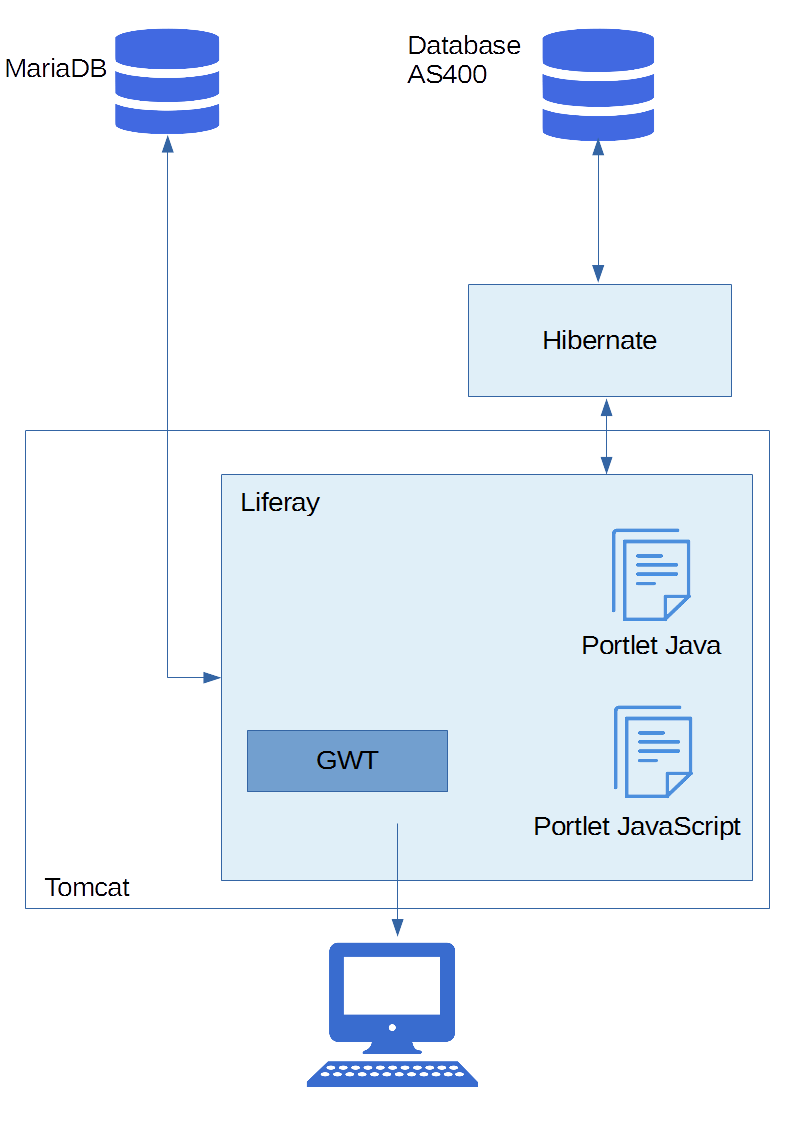
\includegraphics[height = 10 cm]{schema-generale}
	\caption{Schema generale di interconnessione tra le componenti}
	\label{schema-generale}
\end{figure}
L'interazione con le entità di Hibernate avviene per mezzo di Liferay, che si occupa anche della gestione degli accessi degli utenti alla pagina, introducendo il concetto di Single Sing On, e della corretta visualizzazione delle \gls{portlet} all'interno delle pagine del portale. Queste sono caricate di volta in volta, tramite dei servizi REST, dal server Tomcat e possono essere scritte in AngularJS, come ad esempio la \gls{portlet} per la geolocalizzazione o quella che gestisce la timeline, oppure in Java per essere successivamente tradotte in JavaScript tramite i servizi offerti da GWT.\\
Le azioni dell'utente vengono gestite poi da Liferay, che si occupa anche del routing tra le varie pagine del portale. Nel caso ci fossero dei dati da salvare, come nel caso dell'inserimento di un nuovo lead, vengono lanciati dei servizi REST che andranno ad interfacciarsi con le entità gestite da Hibernate, il quale gestisce la persistenza dei dati.\\

\subsection{Portlet life cycle}
Al fine di capire al meglio come progettare la nuova form, mi sono concentrato sullo studio del ciclo di vita di una \gls{portlet}:\\
L'ambiente in cui una essa viene creata ed utilizzata è denominato \emph{portlet container} che, come suggerisce la parola, è un contenitore che gestisce l'aggregazione tra le \gls{portlet}, mantiene memoria delle preferenze dettate dall'utente su di esse ed inoltre funge da \emph{Controller} tra l'interfaccia utente(\emph{View}) ed i dati (\emph{Model}) nel paradigma di programmazione MVC (Model View Controller), illustrato nella sezione ~\ref{sec:MVC}.\\
\newpage
\begin{figure}[h]
	\centering
	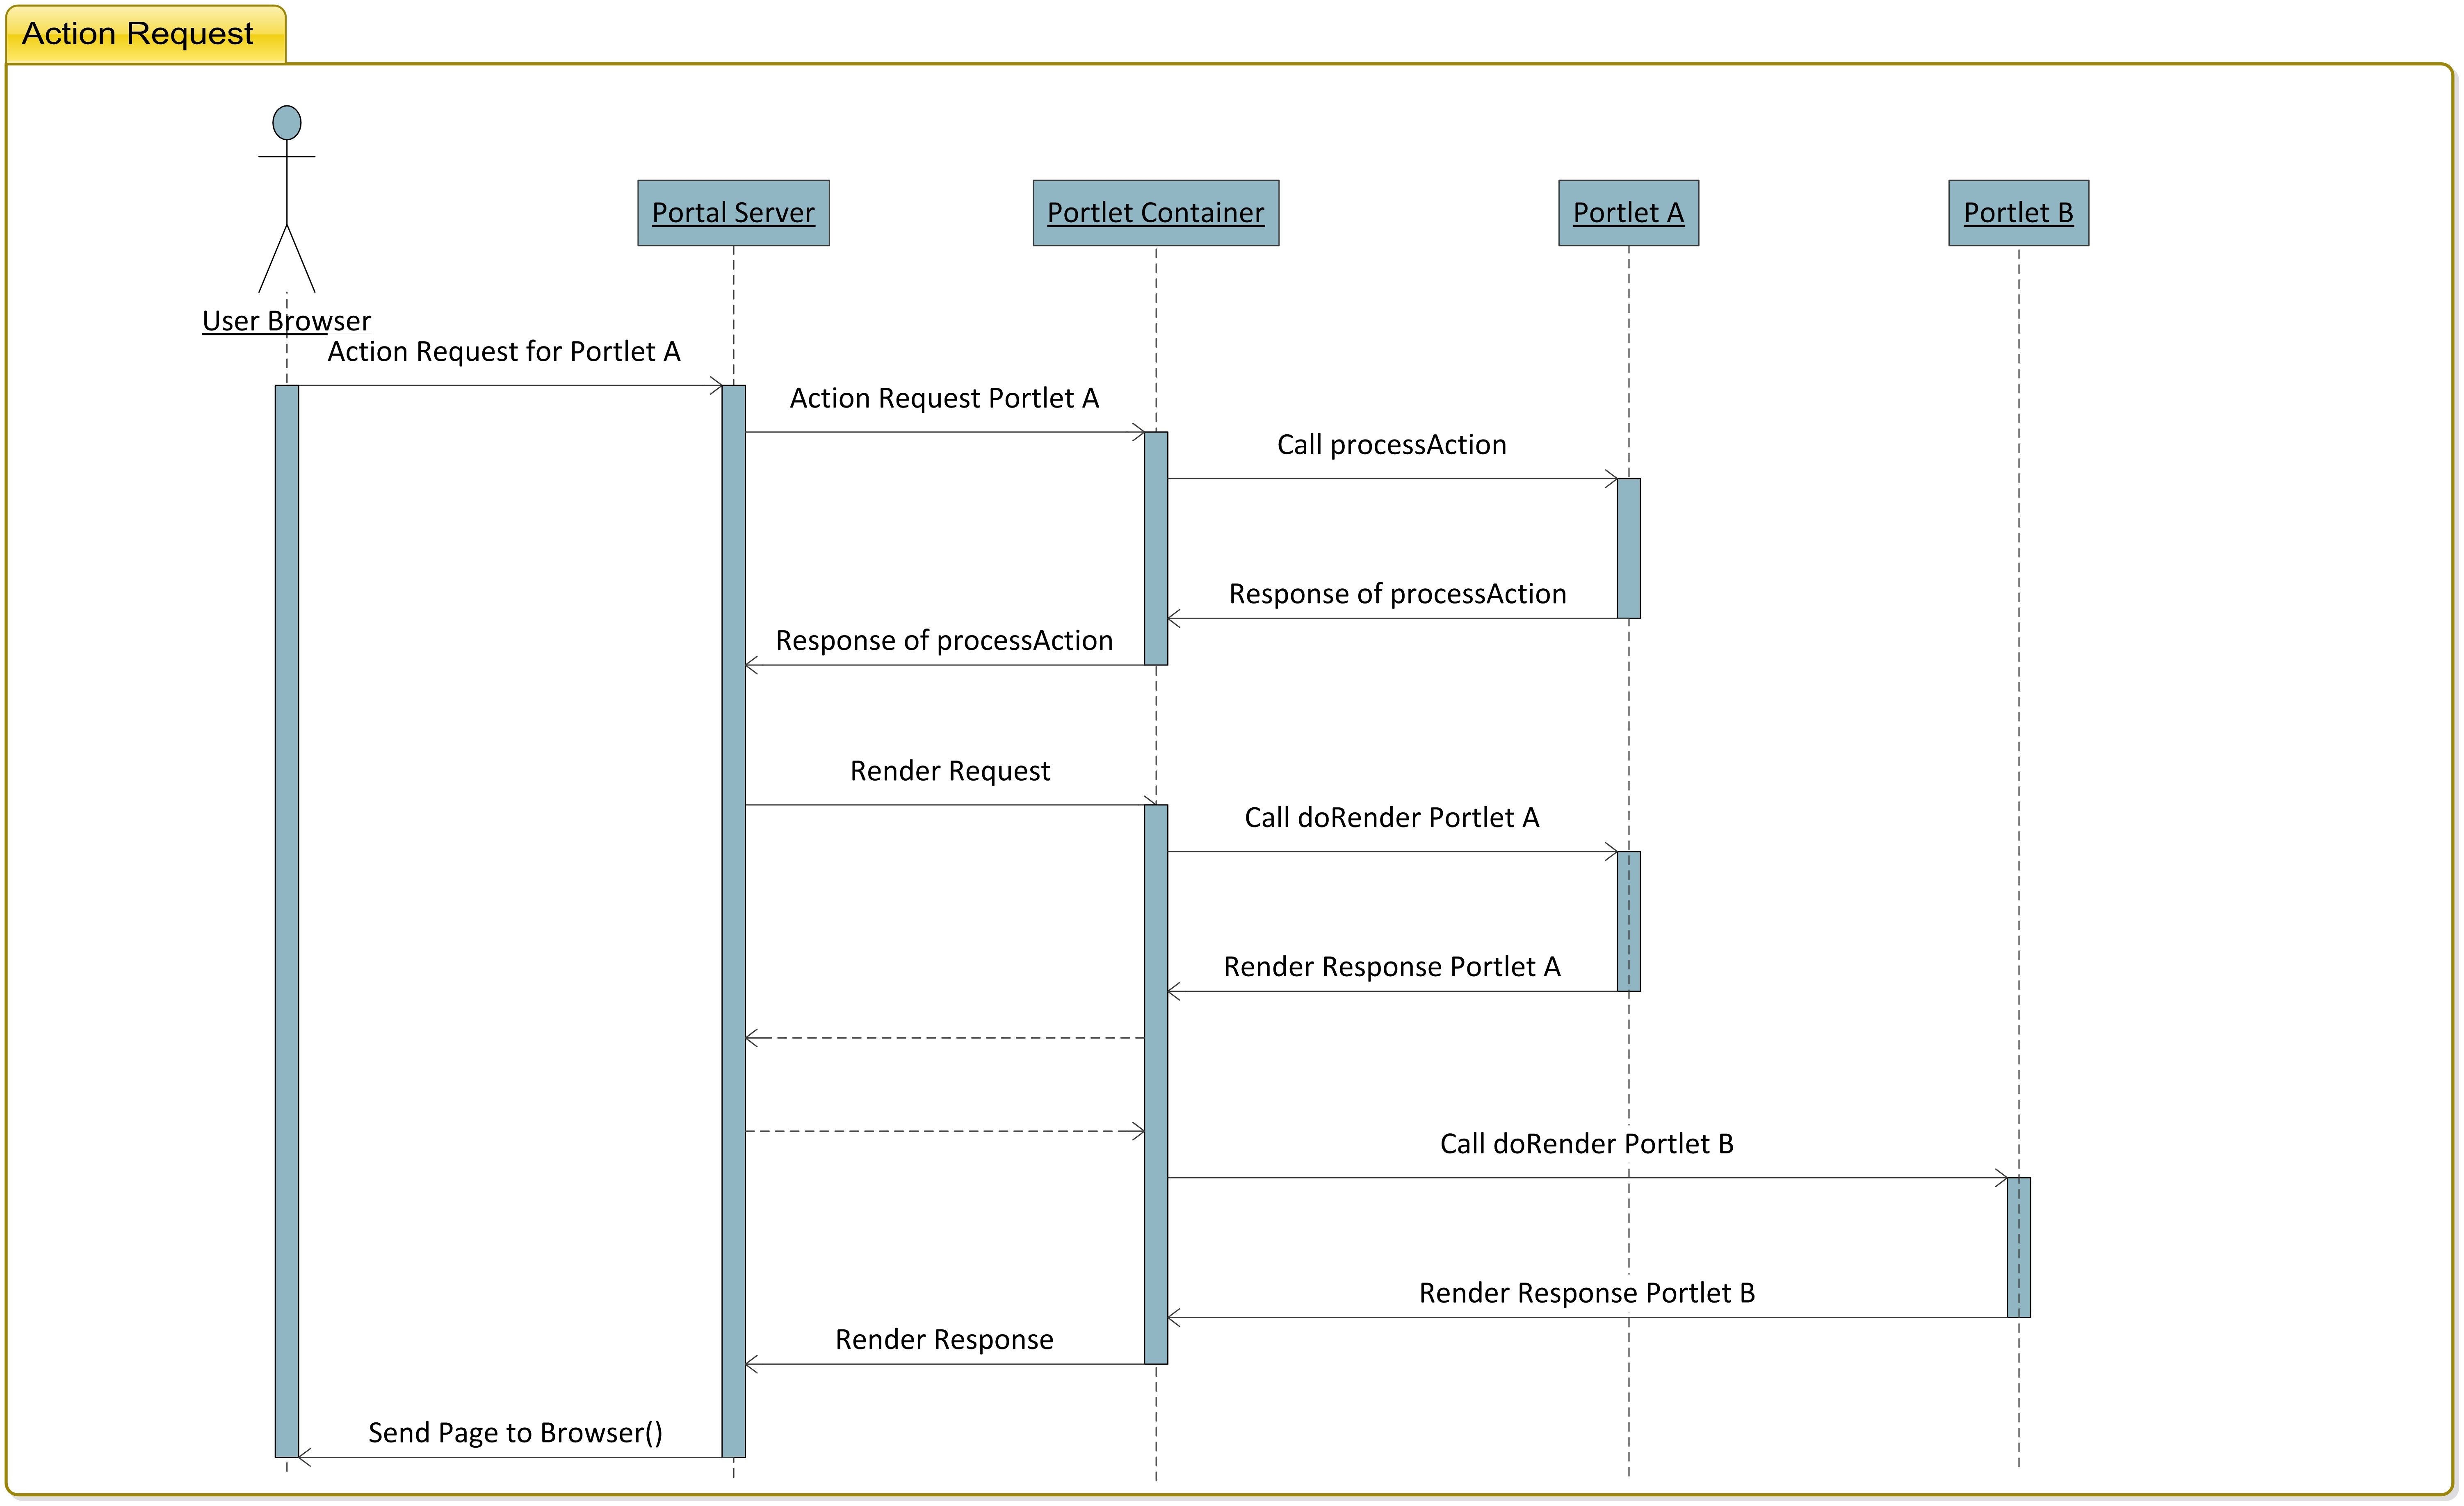
\includegraphics[height = 8 cm]{portet_action_request}
	\caption{Diagramma di sequenza di ProcessAction}
	\label{process-action}
\end{figure}

Il ciclo di vita di una \gls{portlet} è caratterizzato da 6 metodi principali che lo regolano:
\begin{itemize}
	\item \textbf{init()}: chiamato dal portlet container, questo metodo crea la \gls{portlet} desiderata. Durante il ciclo di vita della stassa viene invocato una sola volta;
	\item \textbf{render()}: questo metodo è responsabile della generazione di codice HTML che sarà quindi visualizzato a schermo. Ci sono alcune restrizioni di sicurezza, viene impedita ad esempio la generazione di tag quali <html>, <head>, <body>, che andrebbero a rompere l'intera pagina.
	\item \textbf{processAction()}: processAction viene invocato quando viene eseguita un'azione, ad esempio l'azione di salvataggio di una form. dopo processAction viene automaticamente invocato il metodo render() della portlet e delle altre \gls{portlet}, qualora ve ne fossero.
	\item \textbf{processEvent()}: utilizzato per gestire gli eventi, viene poi chiamato il metodo render() della sola \gls{portlet} interessata;
	\item \textbf{serveRescource()}: metodo utilizzato per reperire risorse utilizzando un \gls{urlg};
	\item \textbf{destroy()}: distrugge la \gls{portlet};
\end{itemize}	
\newpage
\section{Form portlet}
La form la cui reimplementazione costituisce il mio progetto di stage consiste in un unica portlet,scritta in Java. \\
La portlet è costituita da una grande classe, di oltre 6.000 linee di codice, che si appoggia poi ad altre classi per la gestione di aspetti più particolari: ad esempio i campi di tipo picker, cioè dei campi di ricerca che recuperano le voci su cui effettuarla dal database, è separata e lunga circa 4.000 linee di codice.\\
Data l'estrema lunghezza, in rapporto alla mia esperienza di studente, ed alla mancanza di documentazione dovuta all'adozione della metodologia agile, lo studio del funzionamento della portlet che gestisce la form ha richiesto più tempo del previsto. \\ 
L'analisi ha portato allo sviluppo del diagramma di flusso riguardandte la creazione della \gls{portlet}, illustrato nelle figure \ref{form-portlet-flow-diagram-1} e \ref{form-portlet-flow-diagram-2}. Il diagramma è molto generale a causa della grande complessità di metodi e alternative dettate dal fatto che la form viene creata dinamicamente e deve quindi coprire tutte le possibili casistiche in cui è possibile incorrere.\\

\begin{figure}[p]
	\centering
	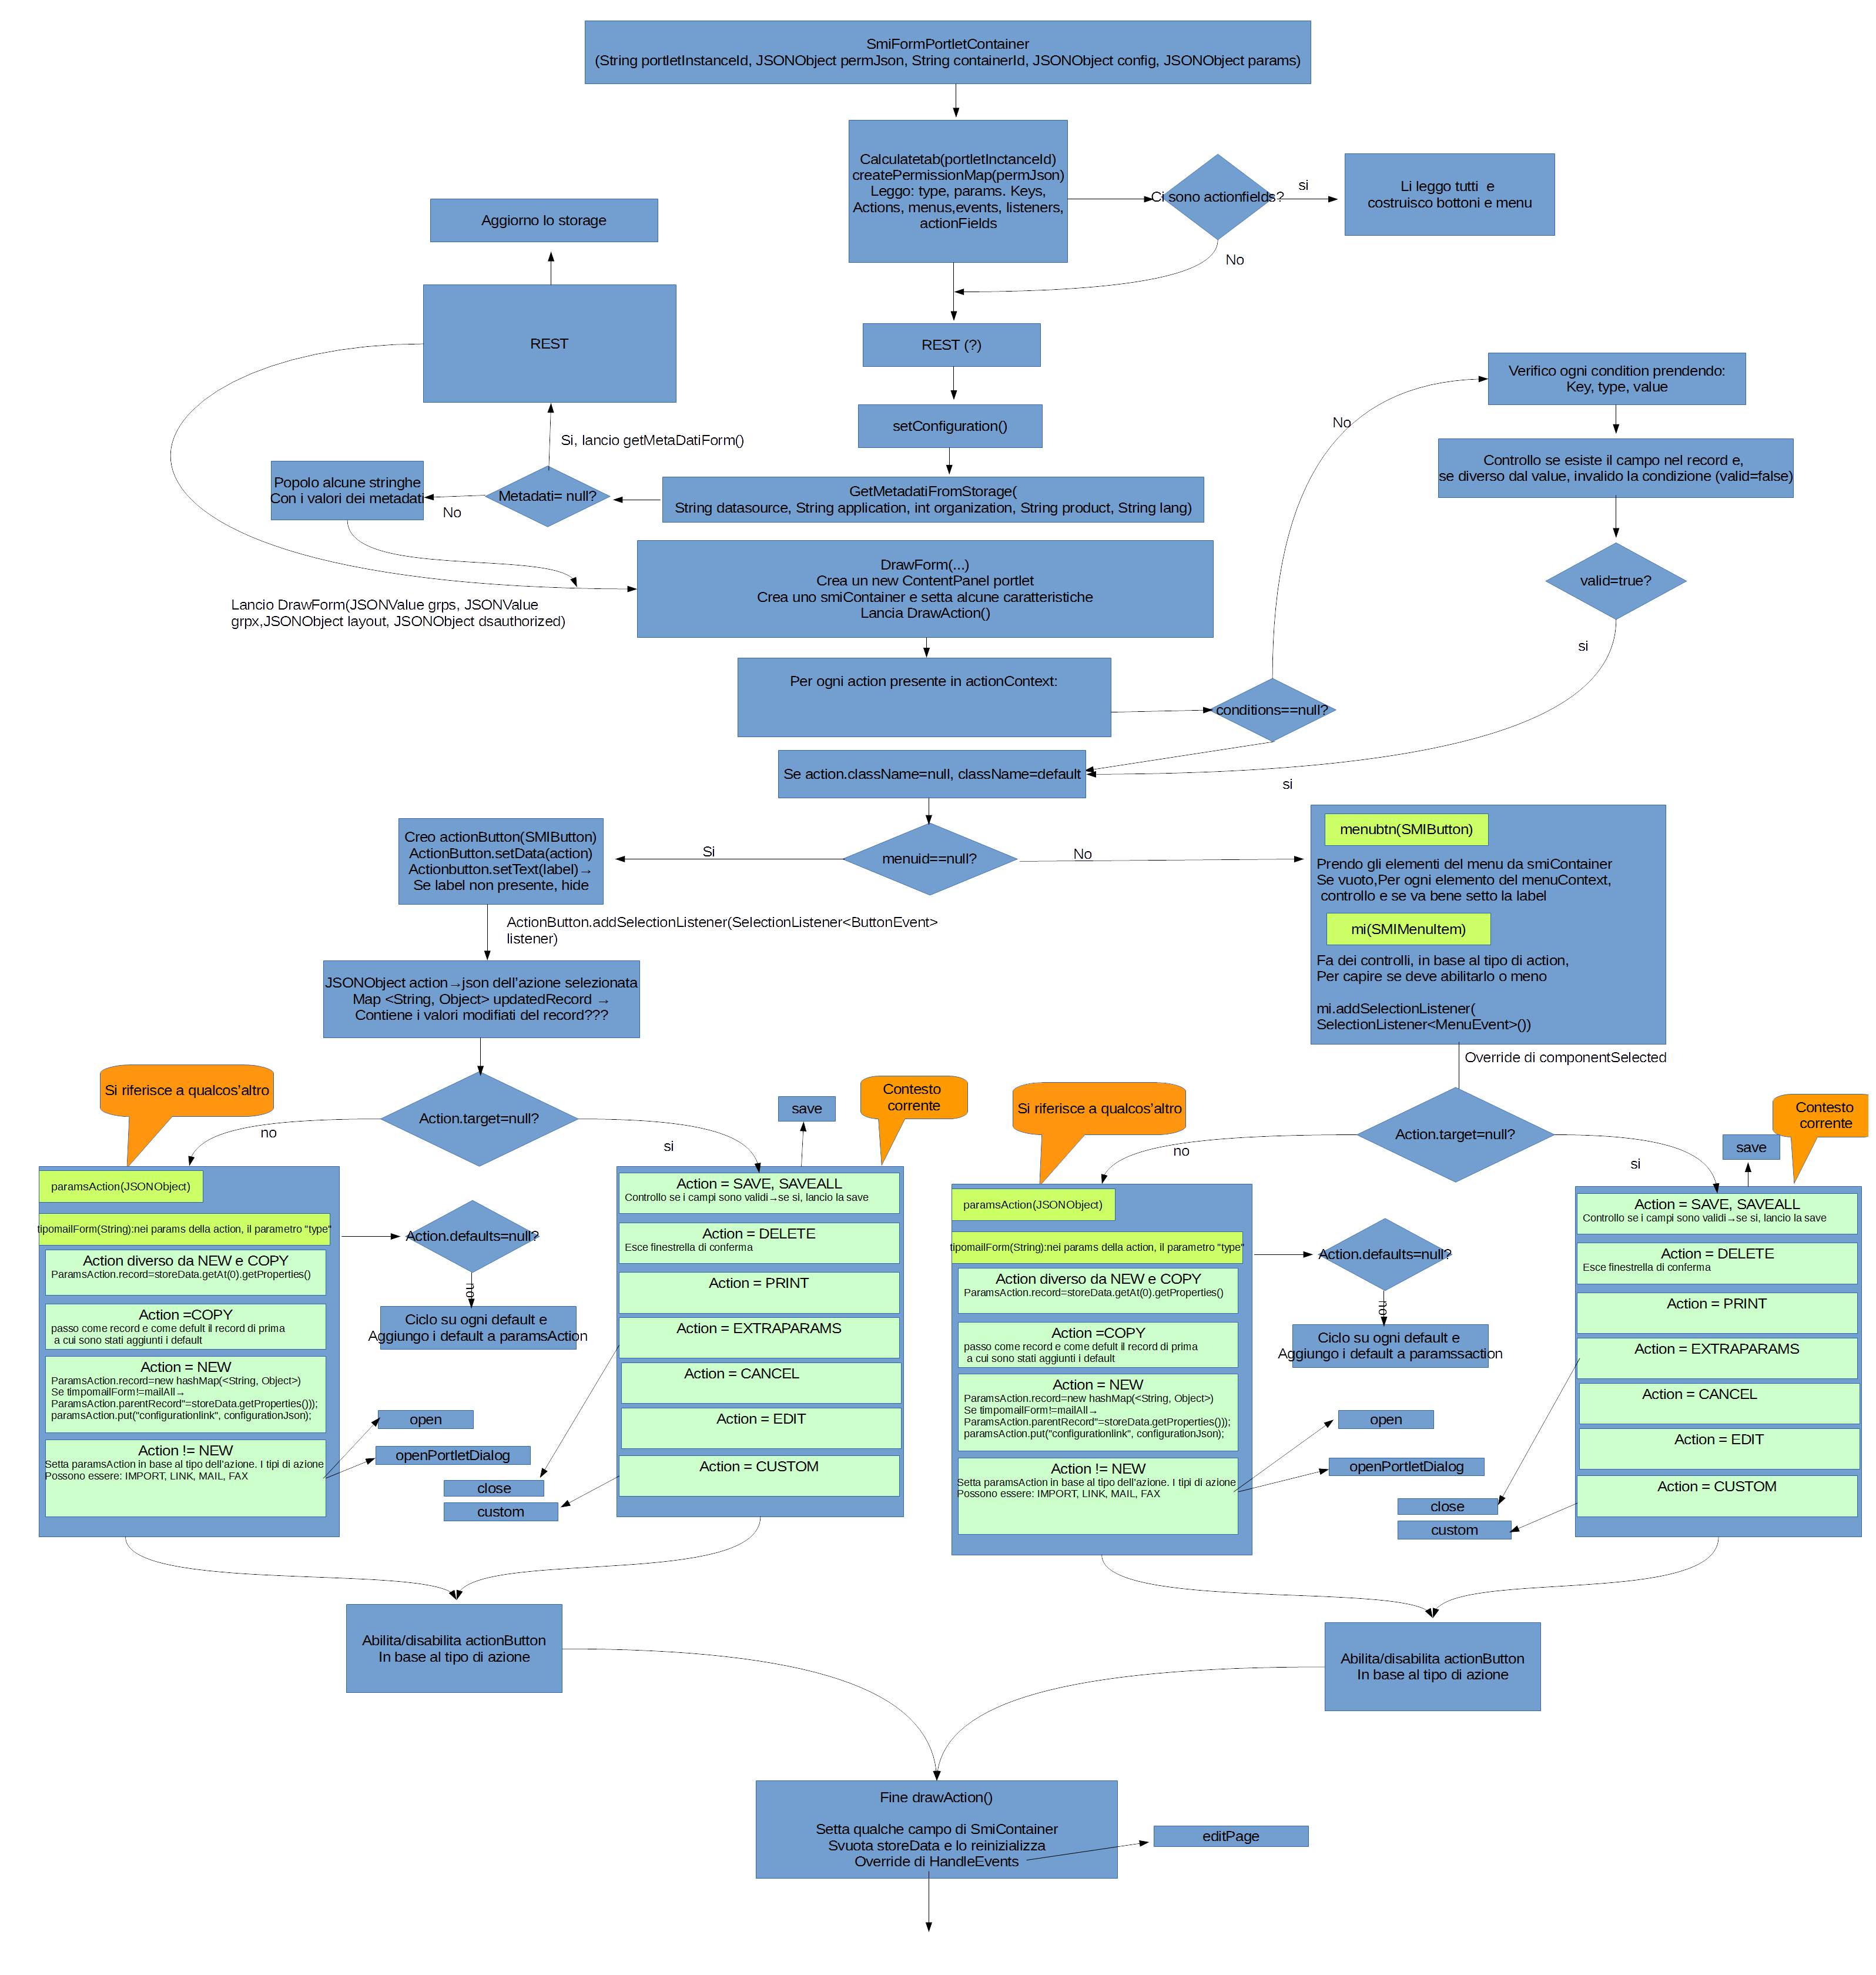
\includegraphics[width=\textwidth, height=\textheight]{diagramma-flusso}
	\caption{Diagramma di flusso della form preesistente- prima parte}
	\label{form-portlet-flow-diagram-1}
\end{figure}

\begin{figure}[p]
	\centering
	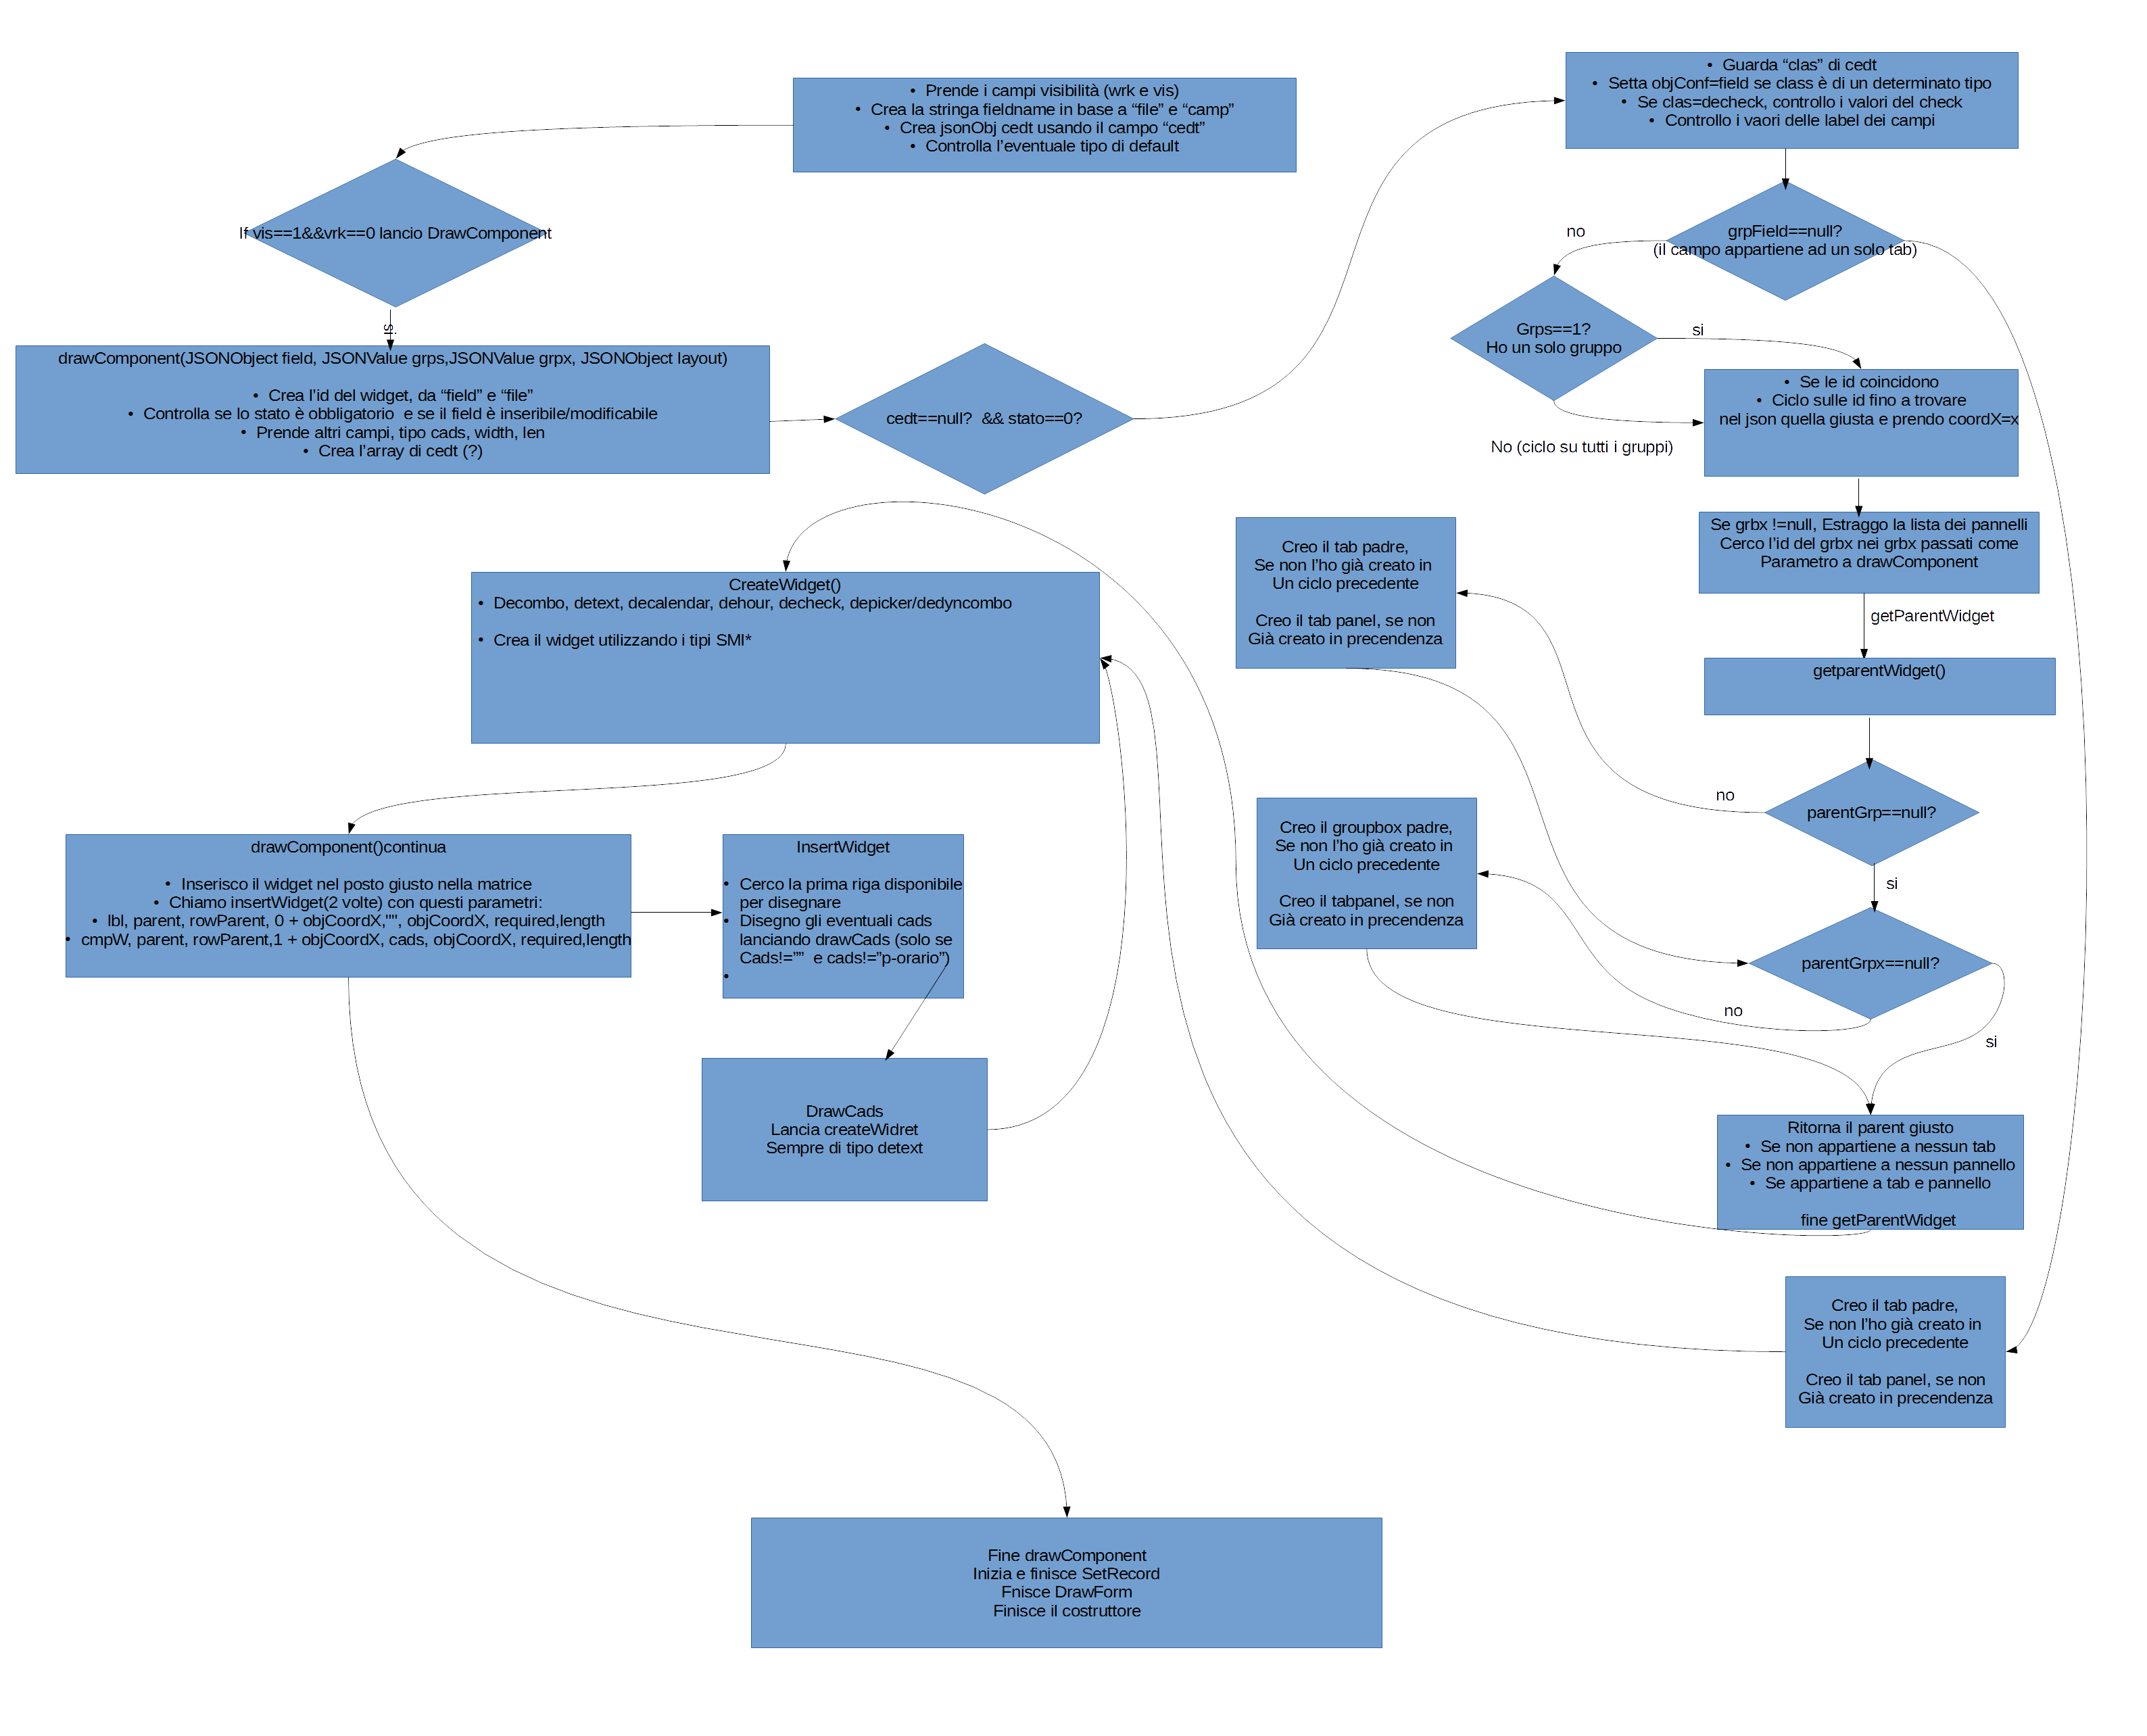
\includegraphics[width=\textwidth, height=\textheight]{diagramma-flusso-ciclo}
	\caption{Diagramma di flusso della form preesistente - seconda parte}
	\label{form-portlet-flow-diagram-2}
\end{figure}

\subsection{Descrizione del flusso}
Il flusso di esecuzione per la creazione di una form può essere essenzialmente diviso in 4 parti: 
\begin{itemize}
	\item \textbf{settaggio dei parametri e costruzione dei bottoni};
	\item \textbf{recupero del datasource};
	\item \textbf{creazione delle azioni};
	\item \textbf{creazione dei fields descritti dal datasource};
\end{itemize}
\subsubsection{Settaggio dei parametri e costruzione dei bottoni}
In questa prima parte del flusso, vengono settati alcuni parametri utili alla creazione della portlet stessa.\\
Al costruttore della classe vengono infatti passati alcuni parametri, contenuti in oggetti di tipo String od in file JSON, contenenti informazioni quali ad esempio:
\begin{itemize}
	\item l'utente connesso con i relativi permessi;
	\item l'id della portlet;
	\item la configurazione della portlet, contenente parametri utili al recupero del datasource;
	\item il \gls{record} dei dati (vuoto nel caso di una form per l'inserimento di dati).
\end{itemize}
Dalla configurazione si prelevano poi parametri sulla presenza o meno di chiavi per il recupero di un \gls{record} in particolare, delle portlet eventualmente in ascolto di cambiamenti e parametri che indicano la presenza di bottoni, che vengono eventualmente costruiti immediatamente.\\
\subsubsection{Recupero del datasource}
Successivamente è necessario recuperare dal server il file JSON contenente l'insieme dei campi dati da visualizzare: viene dapprima controllato se esso è già disponibile nel localStorage e, nel caso esso non fosse già stato caricato in precedenza, viene richiesto al server Tomcat.
La richiesa avviene attraverso delle chiamate REST: %todo
\subsubsection{Creazione delle azioni}
Una volta ottenuto il datasource, è possibile passare alla costruzione delle parti che andranno ad interagire con l'utente:\\
Dapprima vengono lette dal datasource le azioni che la form può eseguire. Il flusso di esecuzione qui si dirama molto a seconda che l'azione abbia o meno una seconda portlet target, che sia contenta o meno in un menù e comunque in base al tipo di azione che si dovrà creare.\\
I tipi di azione sono i seguenti:
\begin{itemize}
	\item \textbf{new};
	\item \textbf{copy};
	\item \textbf{import};
	\item \textbf{link};
	\item \textbf{mail};
	\item \textbf{save};
	\item \textbf{print};
	\item \textbf{delete};
	\item \textbf{custom};
\end{itemize}
I metodi invocati sono diversi per ogni azione, e si occupano della gestione della funzionalità allorché l'utente prema il relativo pulsante.
\newpage
\subsubsection{Creazione dei fields}
Infine viene eseguito un ciclo su tutti i campi dati rappresentati nel datasource. Questa è la parte più complessa del flusso in quanto ogni campo contiene avariate caratteristiche che è necessario andare a verificare per la corretta costruzione dello stesso. Esso è descritto nel datasource, con alcune variazioni (a volte piuttosto importanti) a seconda della tipolgia di campo, come riportato nella figura \ref{fig:json-detail}, che rappresenta i parametri relativi al campo "mail".\\  
	\begin{figure}[h]
		\centering
		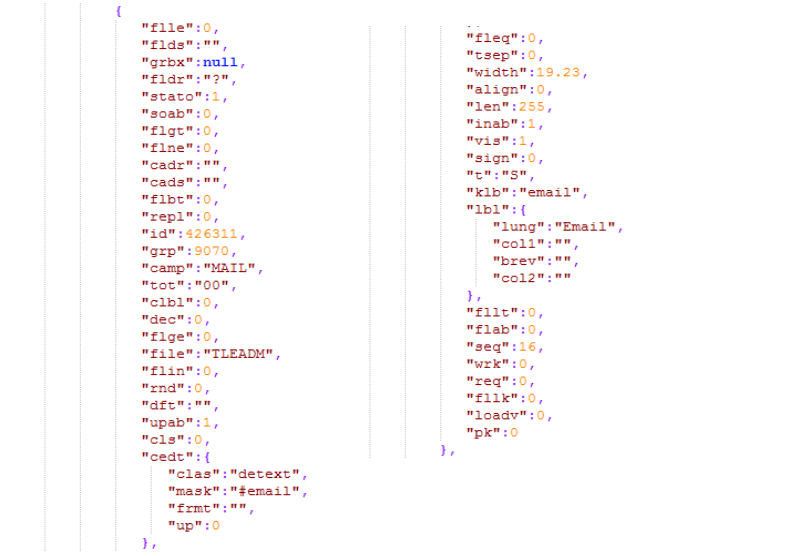
\includegraphics[height=8 cm]{json-details}
		\caption{Esempio di un campo dati come rappresentato nel datasource}
		\label{fig:json-detail}
	\end{figure}
Vengono letti i campi relativi all'effettiva rappresentazione sullo schermo del campo, i premessi di scrittura, l'eventuale valore di default, che viene inserito in un particolare tipo di \gls{record} e vengono letti i valori, rappresentati in un punto differente del file, relativi al posizionamento del campo all'interno della form.\\
Vengono quindi create le tab ed i groupbox per contenere i campi.\\
Viene poi letta la tipologia di campo, che può essere
\begin{itemize}
	\item \textbf{text};
	\item \textbf{combobox};
	\item \textbf{date};
	\item \textbf{picker};
\end{itemize}
Per ognuna di queste tipologie vengono chiamati dei metodi appropriati che costruiscono il campo: il più complesso è il campo picker, che tra i suoi parametri contiene le indicazioni per il recupero dei dati che saranno poi oggetto della ricerca da parte dell'utente.\\
Infine viene effettuata un'ulteriore chiamata REST per recuperare il record completo, tenendo anche conto dei valori di default recuperati dal ciclo appena effettuato.

\newpage             % Concept Preview
% !TEX encoding = UTF-8
% !TEX TS-program = pdflatex
% !TEX root = ../tesi.tex

%**************************************************************
\chapter{Sviluppo del prototipo}
\label{cap:sviluppo-prototipo}
%**************************************************************

\intro{Questo capitolo illustra il funzionamento delle tecnologie che ho utilizzato nello sviluppo del prototipo, la logica di realizzazione ed il risultato ottenuto}\\

%**************************************************************
\section{AngularJS}
\label{sec:AngularJS}

La libreria che ho scelto di utilizzare, AngularJS, nasce nel 2012 nei laboratori di Google.\\
Esso potenzia l'aspetto dichiarativo del linguaggio \gls{html}, offrendo al contempo tutti gli strumenti necessari alla realizzazione di \gls{spag}. 
\subsection{Direttive e controller}
Una delle peculiarità di  AngularJS è che consente di aggiungere al codice HTML nuovi attributi, denominati \textbf{direttive}.\\
Tali direttive possono essere definite dall'utente, che comunque ha a disposizione anche un buon numero di 
direttive standard fornite dal \emph{framework}. Queste strutture consentono al compilatore HTML di AngularJS (attivate dal comando \lstinline[language=Java]!$compile()!, di creare un legame tra l'attributo in cui sono inserite ed il codice JavaScript che va ad eseguire il corpo della direttiva, tipicamente una funzione.\\
La possibilità di definire direttive customizzate estende di molto le funzionalità di base, lasciando alla fantasia del programmatore la creazione di strutture pensate appositamente per l'applicazione in sviluppo, ed consente di utilizzare quasi esclusivamente l'HTML per la creazione delle interfacce grafiche.\\
L'invocazione delle direttive può avvenire utilizzando il nome della direttiva come tag(\lstinline[language=HTML]!<direttiva></direttiva>!), oppure come attributo ad un tag regolare HTML(\lstinline[language=HTML]!<div direttiva></div>!).\\
Nel mio progetto ho utilizzato esclusivamente direttive standard di AngularJS, che ne ha create di specifiche per la creazione di form.\\
\\
L'altro importante componente di AngularJS è il controller. Esso viene invocato tramite la direttiva\lstinline[language=HTML]!ng-controller! ed il suo scope concerne tutto ciò che si trova all'interno dei tag nei quali è definito. Un controller, grazie al concetto di dependency injection, può utilizzare le funzionalità definite in moduli esterni che vengono inseriti come dipendenza all'interno del controller.\\ \'E possibile importare, oltre ad interi metodi, anche singoli oggetti: il più utilizzato è sicuramente l'oggetto di sistema  \lstinline[language=HTML]!$scope!. Quest'ultimo è un semplice oggetto JavaScript, per cui è possibile aggiungervi nuovi attributi e metodi semplicemente digitando \lstinline[language=HTML]!$scope.nuovoattributo = valore;!. Lo scope, assieme alle funzionalità definite nei moduli dichiarati come dipendenza, funge da \emph{model} nel patter MVC descritto in \ref{sec:MVC}.\\
Gli attributi dello \lstinline[language=HTML]!$scope! definiti in un controller sono condivisi all'interno della view (quindi nel codice HTML) unicamente nell'area in cui è definito il controller. AngularJS implementa infatti il concetto di \textbf{two-ways data binding}: il data binding è il meccanismo di sincronizzazione automatica dei dati tra il modello e la view. La maggior parte dei sistemi di template supporta il data binding in una sola direzione, tipicamente dal modello dei dati verso la view. Questo vuol dire che i dati del modello vengono combinati con il template HTML per generare la view visibile all’utente. Se però il modello viene modificato, le modifiche non si riflettono automaticamente sulla view. Analogamente, se l’utente modifica la view, queste modifiche non vengono automaticamente riportate sul modello dei dati. Per sincronizzare view e modello occorre in genere scrivere del codice che lo faccia.\\
Il data binding di AngularJS invece è bidirezionale, cioè ogni modifica al modello dei dati si riflette automaticamente sulla view e ogni modifica alla view viene riportata sul modello dei dati.\\
Per poter utilizzare un attributo dello \lstinline[language=HTML]!$scope! nella view è sufficiente indicarlo, all'interno di un tag di testo, con la seguente sintassi: \lstinline[language=Java]!ng-model = nuovoattributo!. Questa sintassi attiva il cosiddetto \emph{ciclo di digest}.

\subsection{Ciclo di digest}
Il ciclo di digest è ciò che permette di avere il two ways data binding. Ogni volta che viene usata la sintassi \lstinline[language=Java]!ng-model = nuovoattributo!, viene automaticamente creato un \textbf{watch} che ascolta i cambiamenti del valore della variabile a cui è associato, nel nostro caso la variabile "nuovoattributo".\\
Quando viene cambiato il valore di una variabile, il \emph{ciclo di digest} controlla tutti i watch presenti nell'applicazione e, nel caso verifichi il cambiamento di alcune variabili rispetto al ciclo precedente, esegue delle operazioni al fine di aggiornare il DOM nei punti in cui essa è utilizzata.\\
Nel caso di variabili che vengono modificate all'interno di un watch, ad esempio perchè il valore di una variabile dipende dal valore di un'altra, il ciclo viene ripetuto finchè non si presentano più modifiche.\\
Questo avviene in maniera del tutto automatica e trasparente sia all'utente che allo sviluppatore, che può però creare dei watch attraverso l'attributo di sistema \lstinline[language=Java]!$watch(attribute, function([data]){})!.\\ Questo nel caso ci siano delle dipendenze da rispettare, ma non ci sia alcun binding con la view. Nel mio progetto, ad esempio, utilizzo questa funzionalità per poter gestire le chiamate asincrone ai servizi REST, sfruttando il cambio di valore della variabile da recuperare.


\subsection{Eventi} 
Gli attributi assegnati allo \lstinline[language=HTML]!$scope! non sono comunque strettamente ristretti al controller in cui sono definiti: è infatti possibile il passaggio degli attributi tra controller annidati come avviene in un comune contesto di ereditarietà: un controller figlio eredita tutti gli attributi definiti nel controller padre.\\ 
Nel contesto di una gerarchia di controller è anche possibile sollevare degli eventi sia un controller figlio a quello padre, utilizzando \lstinline[language=HTML]!$emit('event name', [data])!, che dal padre verso i figli, con \lstinline[language=HTML]!$broadcast('event name', [data])!.\\
Gli eventi vengono poi raccolti da \lstinline[language=HTML]!$on('event name', function([data]){...})!, che definisce il comportamento da adottare una volta raccolto l'evento.\\

\section{Codifica}
La creazione della componente form utilizzando angularJS è iniziata cercando di aderire ai principî dell'incapsulamento e di \emph{information hiding} tipici della programmazione ad oggetti.\\ Questi principî, che sanciscono la necessità di nascondere le proprietà intrinseche di un oggetto rispetto alla sua rappresentazione, sono qui utilizzati per separare i compiti tra i diversi elementi della form tramite l'utilizzo di vari controller, ognuno destinato alla gestione di una porzione specifica della form stessa.\\
Vengono quindi utilizzati dei controller generici, che vengono instanziati una sola volta:
\begin{itemize}
	\item \textbf{FormController}: un controller generale, che recupera le informazioni utili alla form nel suo complesso, come record e datasource;
	\item \textbf{ActionsController}: un controller che gestisce la creazione delle azioni e il loro comportamento; indipendente dall'altro;
	\item \textbf{FieldsController}: un controller che si occupa della creazione dei campi dati che costituiscono il corpo della form.
\end{itemize}
e specifici in cui, per ogni button del tipo interessato, viene instanziato un nuovo controller:
\begin{itemize}
	\item controller figli di ActionsController:
	\begin{itemize}
		\item \textbf{ActionButtonController}: un controller per gestire il singolo button d'azione;
	\end{itemize} 
	\item controller figli di FieldsController:
	\begin{itemize}
		\item \textbf{PickersController}: un controller per il controllo dei campi di tipo picker;
		\item \textbf{DetextController}: un controller per il controllo dei campi di tipo text;
		\item \textbf{GeneralFieldController}: un controller per il controllo dei campi diversi dal tipo picker e text. \\Quest'ultimo, in particolare, è stato pensato in ottica manutentiva: se è necessario aggiungere delle proprietà ad un campo generico, è possibile farlo andando a modificare questo controller.
	\end{itemize} 
\end{itemize} 

\begin{figure}[h]
	\centering
	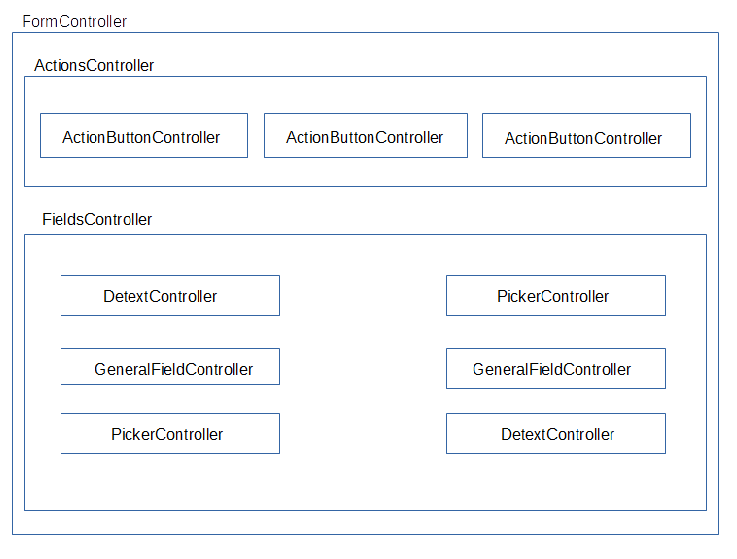
\includegraphics[height=10 cm]{gerarchia-controller}
	\caption{gerarchia di controller in una form}
	\label{fig:ger-contr}
\end{figure}

\subsection{Ciclo di creazione}
\subsubsection{Recupero dei dati}
La creazione di una form avviene seguendo parzialmente il flusso di creazione utilizzato dalla precedente implementazione e visto nel precedente capitolo, ma ho comunque cercato di utilizzare meno risorse possibili per aumentare la velocità di creazione e migliorare l'esperienza utente. La velocità di creazione è inoltre aumentata dalla scelta di caricare dinamicamente alcune componenti della form, come i tab, solamente se l'utente vi interagisce realmente.\\
La direttiva \lstinline[language=HTML]!ng-app!, che inizializza l'applicazione AngularJS, può essere utilizzato solamente una volta all'interno di un documento HTML: in JGalileo CRM era già utilizzata per inizializzare un modulo comune, chiamato SMICommonModule, che conteneva anche alcuni servizi REST per il reperimento di risorse quali datasource e record. Tali servizi sono stati successivemente integrati con nuove funzionalità. \'E stato quindi sufficiente importare il modulo come dipendenza del controller principale della form per poter correttamente inizializzare il tutto.\\
Al controller principale vengono passati alcuni parametri di configurazione, con cui viene recuperato il datasource corretto tramite un servizio REST. \\
Tramite il meccanismo di \lstinline[language=HTML]!$watch! descritto in precedenza, al ritorno del datasource
viene chiamato il metodo \lstinline[language=HTML]!setValues()! contenuto in FieldsController, che si occupa di creare degli array contenti le azioni, i tab della form e, per ogni tab, i groupbox che lo conpongono. Successivamente vengono letti tutti i campi dati descritti nel datasource e posti negli array, per facilitarne la rappresentazione.\\ AngularJS mette infatti a disposizione la direttiva \lstinline[language=HTML]!ng-repeat!, che consente di iterare lungo una lista od un array di elementi. \\
\begin{figure}[h]
	\centering
	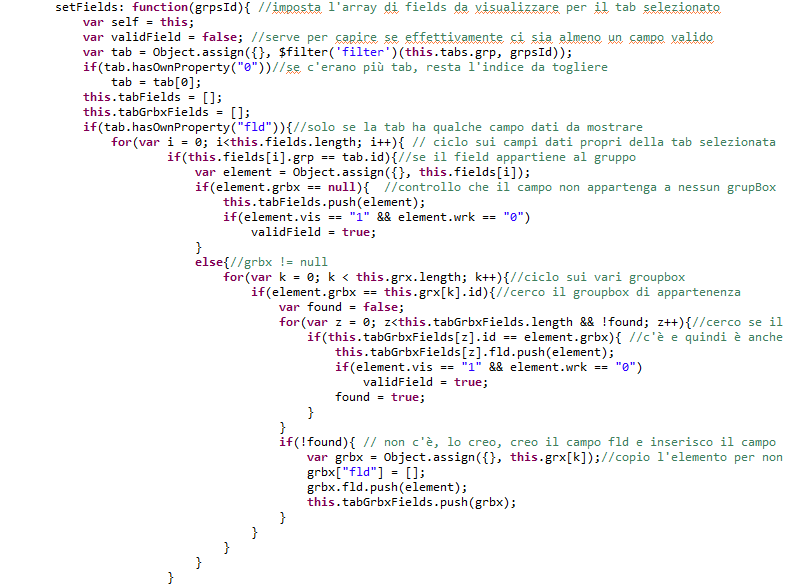
\includegraphics[height=8 cm]{setFields}
	\caption{setFields(), che inserisce i valori negli array}
	\label{fig:set-fields}
\end{figure}
Al termine di queste operazioni, vengono inizializzati nel record i campi contententi i valori di default. Questo record viene poi utilizzato per recuperare dal server il record completo, composto dai campi di default precedentemente settati e da alcuni altri campi che vengono inseriti dal server.\\
Una volta ottenuto il record completo, i valori che sono stati recuperati vengono visualizzati direttamente nella view grazie al \emph{two ways data binding}.

\subsubsection{Creazione della view}
Il file che costituisce la view è unico e rispecchia, utilizzando tag innestati, la gerarchia dei controller vista nell'immagine \ref{fig:ger-contr}\\
\begin{figure}[h]
	\centering
	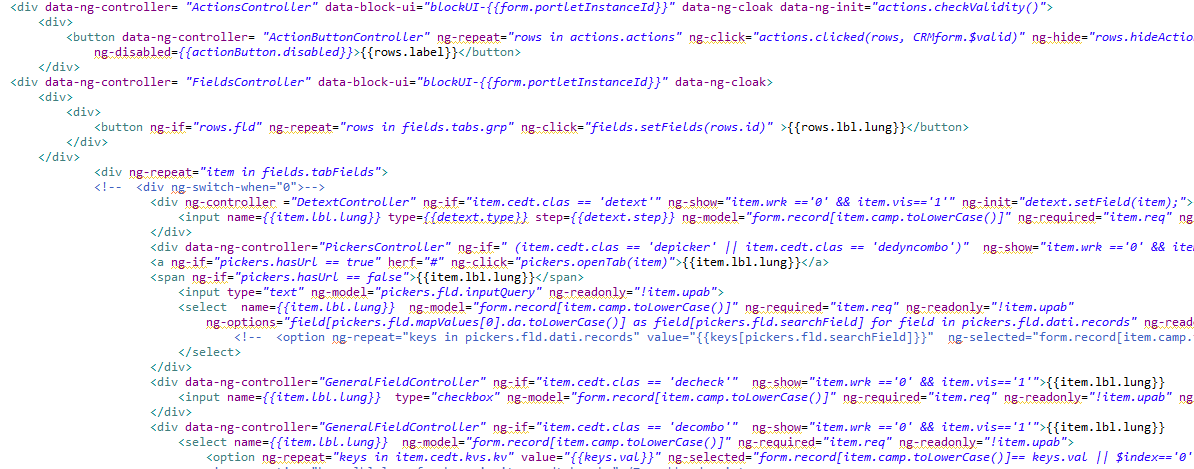
\includegraphics[height=7 cm, width= 15 cm]{view}
	\caption{parte della view}
	\label{fig:view}
\end{figure}

Vengono creati i buttons per le azioni e dei buttons che poi andranno a costituire i tab di cui è composta la form.\\
In seguito il file è essenzialmente diviso in due parti: la prima, che tramite l'esecuzione di un ciclo sull'array corretto si occupa della creazione dei campi dati che non appartengono ad alcun groupbox, e la seconda, che utilizzando due cicli gestisce la creazione delle groupbox e dei campi contenuti in ciascuna di esse.
Nella view sono poi inserite, come attributo di tag, svariate direttive, come il condizionale \lstinline[language=HTML]!ng-if!, \lstinline[language=HTML]!ng-readonly!, \lstinline[language=HTML]!ng-show! che servono alla corretta visualizzazione di un determinato campo dati sulla base delle proprietà descritte per quel campo nel datasource recuperato. \\
Ogni campo della form utilizza la direttiva \lstinline[language=HTML]!ng-model!, in maniera che venga attivato il ciclo di digest per ogni campo, e che il valore descritto da esso venga automaticamente salvato nel record. \\ La sintassi \lstinline[language=HTML]!{{variable}}! viene invece utilizzata per rappresentare a schermo il valore della variabile \lstinline[language=HTML]!variable!. Nel mio progetto queta direttiva è utilizzata per visualizzare il nome del campo.

\subsection{Validazione dei campi inseriti}

AngularJS mette a disposizione molte funzionalità dedicate alla realizzazione di form.\\
Una di queste è la validazione della form a livello client. AngularJS, in maniera del tutto autmatica, valuta se i dati inseriti siano del tipo dichiarato per ogni campo e se vengono rispettate le obbligatorietà. Un campo viene dichiarato obbligatorio tramite la direttiva \lstinline[language=HTML]!ng-required! \\
La validazione dell'intera form è possibile racchiudendo la form stessa in un tag HTML \lstinline[language=HTML]!<form>! ed utilizzando la proprietà \lstinline[language=HTML]!valid()! su di esso. L'interà form sarà valida solo se tutti i campi della form sono validi.	\\
La validazione viene utilizzata nell'interazione con le azioni per essere sicuri che i campi che andranno inseriti nel sistema rispettino i vincoli dati loro. Altri controlli vengono comunque eseguiti lato server, prima di effettuare l'inserimento dei dati.


\subsection{Difficoltà nello sviluppo}
Lo sviluppo della form oggetto del mio progetto di stage è andata incontro anche ad alcune problematiche che hanno impedito il completo soddisfacimento dei requisiti: in particolare, in due occasioni il tempo impiegato per cercare di superare le problematiche è stato consistente:
\begin{itemize}
	\item \textbf{\$http}: questo servizio consente di effetturare chiamate \gls{ajaxg} per il recupero di dati in maniera asincrona dal server.\\
	Questo servizio ha funzionato egregiamente con i dati recuperati da FormController, come il recupero di record e datasource, ma aveva un comportamento piuttosto altalenante, con la quasi totalità di richieste fallite, nel recupero di dati da controller figli. In particolare, i dati dei campi di tipo picker risultavano praticamente impossibili da recuperare nel momento dell'interazione con l'utente.\\
	In accordo col tutor, è stato eseguito un refactoring per fare in modo di recuperare tutti i dati nel momento della creazione dell'intera form. Questa soluzione è parsa però da subito estremamente inefficente, in quanto era necessario caricare tutti i dati di tutti i campi eventualmente inseribili dall'utente, che per alcuni campi superano le migliaia di unità. \\
	La soluzione è arrivata sostituendo il servizio \lstinline[language=HTML]!$http()! con il più generico \lstinline[language=HTML]!$.ajax()!, dopo svariati giorni di tentativi nell'utilizzo di soluzioni alternative e di test per comprendere la causa del comportamento anomalo del servizio;
	\item \textbf{vendors}: un vendor, nella struttura di JGalileo CRM, rappresenta un pacchetto esterno installabile ed utilizzabile all'interno di un modulo: in quest'ottica ho cercato di inserire il pacchetto definito \href{https://github.com/angular/material}{angularjs-material} tra i pacchetti utilizzabili nella form. Purtroppo il metodo di installazione classico, descritto anche nell'URL appena riportato, non era utilizzabile in quanto non è stato possibile risalire alla sezione head del documento.\\ Pur provando svariate soluzioni alternative, nessuna di esse ha funzionato e nè il tutor nè il resto del team è stato in grado di aiutarmi nel superamento del problema, che pertanto ad oggi è rimasto insoluto e non mi ha permesso di inserire dello stile nel progetto. La creazione di un foglio di stile da zero sarebbe infatti risultato troppo oneroso in termini di tempo e difficoltoso nella realizzazione, in quanto ogni groupbox contiene un numero di colonne definito nel datasource ed i campi dati sono posizionati in base ad esse.
\end{itemize}
\newpage
             % Product Prototype
% !TEX encoding = UTF-8
% !TEX TS-program = pdflatex
% !TEX root = ../tesi.tex

%**************************************************************
\chapter{Conclusioni}
\label{cap:conclusioni}
%**************************************************************

\intro{}

\section{Produttività}
Nel piano di lavoro concordato con l'azienda all'inizio dell'esperienza sono stati definiti degli obiettivi di tipo formativo e produttivo che avrei dovuto raggiungere, mentre nel corso dello stage sono stati da me definiti i reauisiti che il prodotto avrebbe dovuto soddisfare. La tabella \ref{tab:obiettivi-raggiunti} riassume gli obiettivi formativi e produttivi raggiunti al termine dello stage, mentre la tabella \ref{tab:obiettivi-riepilogo} riassume il numero di requisiti obbligatori, desiderabili ed opzionali che sono stati completati nel corso dello stage:\\

\subsection{Raggiungimento degli obiettivi personali}
\begin{table}[h]
	\centering
	\caption{Obiettivi dello stage}
	\label{tab:obiettivi-raggiunti}
	\begin{tabular}{|l|c|p{7cm}|p{4cm}|}
		\hline
		\rule[-4mm]{0mm}{1cm}
		ID & Importanza & Descrizione & Soddisfatto\\
		\hline
		\rule[-3mm]{0mm}{0.8cm}
		F1 & Obbligatorio & Acquisizione delle competenze di base sulla famiglia di software denominata CRM. & Soddisfatto\\
		\hline
		\rule[-3mm]{0mm}{0.8cm}
		F2 & Obbligatorio & Acquisizione delle competenze di base sul software di sviluppo GWT. & Soddisfatto\\
		\hline
		\rule[-3mm]{0mm}{0.8cm}
		F3 & Desiderabile & Acquisizione di competenze avanzate sul linguaggio di programmazione utilizzato per lo sviluppo del prototipo. & Soddisfatto\\
		\hline
		\rule[-3mm]{0mm}{0.8cm}
		P1 & Obbligatorio & Analisi dei requisiti tecnici ed applicativi. & Soddisfatto\\
		\hline
		\rule[-3mm]{0mm}{0.8cm}
		P2 & Obbligatorio & Analisi dell'User Interface. & Soddisfatto\\
		\hline
		\rule[-3mm]{0mm}{0.8cm}
		P3 & Obbligatorio & Analisi degli Use Case. & Soddisfatto\\
		\hline
		\rule[-3mm]{0mm}{0.8cm}
		P4 & Obbligatorio & Sviluppo di un prototipo che implementi le stesse funzionalità del componente esistente. & Soddisfatto\\
		\hline
		\rule[-3mm]{0mm}{0.8cm}
		P5 & Facoltativo & Implementazione di nuove funzionalità di interazione con l'utente sul prototipo sviluppato. & Non soddisfatto\\
		\hline
	\end{tabular}
\end{table}
Complessivamente, tutti gli obiettivi obbligatori e desiderabili sono stati soddisfatti, mentre il requisito non soddisfatto, riguardante lo sviluppo di nuove funzionalità, non è stato soddisfatto a causa di alcuni problemi che sono emersi durante il corso dello stage, diminuendo il tempo a mia disposizione.\\

\subsection{Soddisfacimento dei requisiti}
\begin{table} %todo
	\centering
	\caption{Riepilogo del soffisfacimento rei requisiti}
	\label{tab:obiettivi-riepilogo}
	\begin{tabular}{|p{2,5cm}|p{2,5cm}|p{2,5cm}|p{2,5cm}|p{2,5cm}|}
		\hline
		\rule[-4mm]{0mm}{1cm}
		\textbf{Tipo} & \textbf{Obbligatorio} & \textbf{Facoltativo} & \textbf{Desiderabile} & \textbf{Soddisfatti}\\
		\hline
		\rule[-3mm]{0mm}{0.8cm}	
		\textbf{Funzionali} & 59 & 0 & 2 & 60\\
		\hline
		\rule[-3mm]{0mm}{0.8cm}	
		\textbf{Qualità} & 1 & 0 & 1& 1\\
		\hline
		\rule[-3mm]{0mm}{0.8cm}	
		\textbf{Vincolo} & 2& 0 & 0 & 2\\
		\hline
		\rule[-3mm]{0mm}{0.8cm}		
		\textbf{Totale} & \textbf{62} & \textbf{0} & \textbf{3} & \textbf{63}\\
		\hline	
	\end{tabular}
\end{table}

Complessivamente, la quasi totalità dei requisiti è stata soddisfatta. I motivi che hanno portato al mancato soddisfacimento sono da ricercare nella generale mancanza di tempo e nell'impossibilità ad implementare alcuni moduli esterni, come descritto nel paragrafo \ref{cap:diff_sviluppo}.

\section {Obiettivi personali}
Nell'intraprendere il mio percorso di stage, oltre agli obiettivi stabiliti nel Piano di Lavoro, avevo anche degli obiettivi personali da raggiungere, di seguito elencati:
\begin{itemize}
	\item Conoscere uno dei rami lavorativi in cui è possibile inserirsi al termine del percorso di studi;
	\item Conoscere tecnologie nuove e non affrontate durante il percorso di studi;
	\item Confrontarmi con software di larga scala;
	\item Confrontarmi con altre persone già inserite nel mondo del lavoro;
	\item Migliorarmi grazie all'aiuto del tem di lavoro;
	\item Migliorarmi nella gestione di tempi/risorse nel contesto di un lavoro assegnatomi.
\end{itemize}             % Product Design Freeze e SOP
% !TEX encoding = UTF-8
% !TEX TS-program = pdflatex
% !TEX root = ../tesi.tex

%**************************************************************
\chapter{Conclusioni}
\label{cap:conclusioni}
%**************************************************************

%**************************************************************
\section{Consuntivo finale}

%**************************************************************
\section{Raggiungimento degli obiettivi}

%**************************************************************
\section{Conoscenze acquisite}

%**************************************************************
\section{Valutazione personale}
             % Conclusioni
\appendix                               
% !TEX encoding = UTF-8
% !TEX TS-program = pdflatex
% !TEX root = ../tesi.tex
\null\newpage
%**************************************************************
\chapter{Approfondimenti}
%**************************************************************

\section{Funzionamento di Hibernate} 
\label{sec:appendice-1}
Come avviene la conversione delle tabelle in classi Java?\\
\begin{figure}[h]
	\centering
	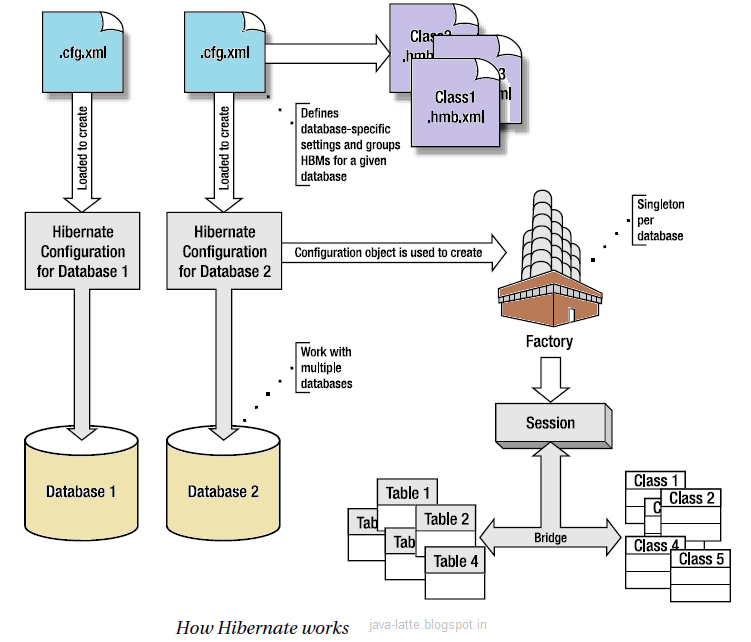
\includegraphics[height = 5 cm]{hibernate_works}
	\caption{Schema del funzionamento di Hibernate}
	\label{schema-generale-hibernate}
\end{figure}
Hibernate deve conoscere la configurazione del database e per farlo necessita di un file, estesi generalmente in \textbf{.cfg.xml}. Al framework è inoltre indispensabile fornire dei files di mapping, uno per ogni tabella e generalmente estesi con i suffissi \textbf{.hmb.xml}, che contengono le informazioni riguardanti le colonne della singola tabella da trasformare in un oggetto Java.\\

\begin{figure}[h]
	\centering
	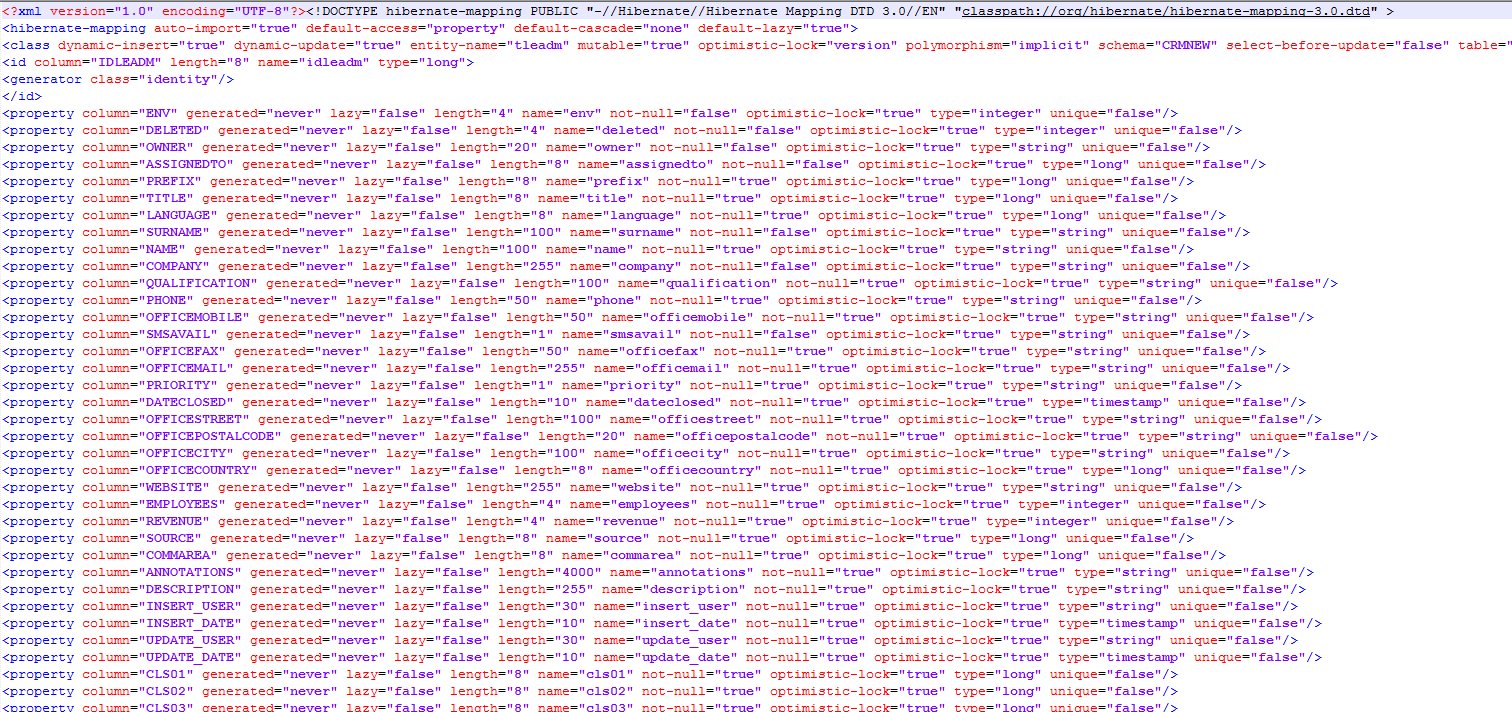
\includegraphics[height = 5 cm]{hibernate-entities}
	\caption{XML di un'entità Hibernate di JGalileo CRM}
	\label{entità}
\end{figure}

Questi files vengono poi utilizzati per creare una \emph{SessionFactory} globale e thread-safe che funge da \emph{gateway} per l'interrogazione del database. \\ I vantaggi dell'utilizzo della tecnica di programmazione ORM (Object-Relational Mapping) sono molteplici ed in particolare consentono:
\begin{itemize}
	\item \textbf{Disaccoppiamento dal DBMS};
	\item \textbf{Elevata portabilità};
	\item \textbf{Drastica riduzione del codice sorgente}, a causa dei semplici comandi che mascherano complesse istruzioni;
	\item \textbf{Elevata modularità}.
\end{itemize}

\section{Model View Controller}
\label{sec:MVC}
Il pattern \emph{MVC, Model-View-Controller}, è un design pattern, cioè uno schema di progettazione che costituisce una soluzione progettuale ad un problema ricorrente \hyperlink{01}{[1]}.\\
\'E uno dei pattern più famosi ed utilizzati per la separazione tra la logica di presentazione e la logica di business nei sistemi software, ed in particolare nelle applicazioni web.\\
\begin{figure}[h]
	\centering
	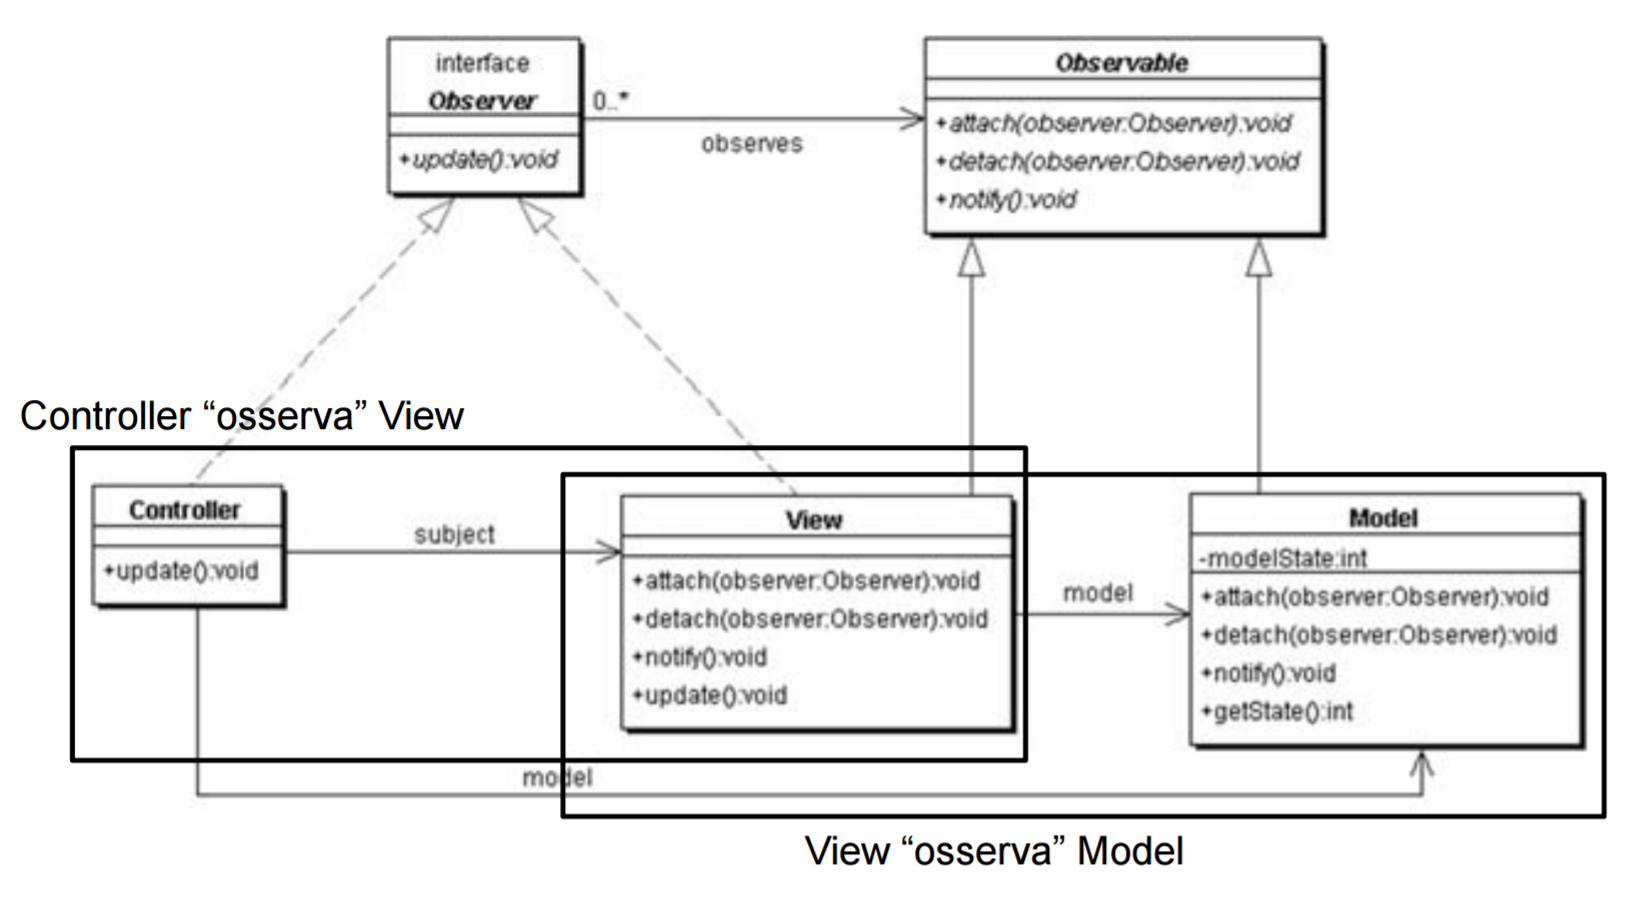
\includegraphics[height = 7 cm]{MVC}
	\caption{Design pattern MVC}
	\label{mvc-schema}
\end{figure}
Come evidenziato dalla figura \ref{mvc-schema}, vi sono 3 attori principali:
\begin{itemize}
	\item \textbf{Model}: rappresenta la cosiddetta \emph{logica di business}, cioè l'insieme di dati e metodi per eseguire operazioni;
	\item \textbf{View}rappresenta come i dati vengono visualizzati nell'interfaccia utente, cioè la \emph{logica di presentazione};
	\item \textbf{Controller}:si pone come intermediario tra view e model;
\end{itemize}
Il controller, che osserva la view, riceve da quest'ultima le richieste di elaborazione e, una volta che il model restituisce i dati, si occupa di inviarli alla view.\\
Questo design pattern ha molti lati positivi, tra i quali la divisione dei compiti ed il riuso di codice.\\


\newpage             % Appendice A

%**************************************************************
% Materiale finale
%**************************************************************
\backmatter
\printglossaries
% !TEX encoding = UTF-8
% !TEX TS-program = pdflatex
% !TEX root = ../tesi.tex

%**************************************************************
% Bibliografia
%**************************************************************

\cleardoublepage
\chapter{Bibliografia}

\nocite{*}
% Stampa i riferimenti bibliografici
\printbibliography[heading=subbibliography,title={Riferimenti bibliografici},type=book]

% Stampa i siti web consultati
\printbibliography[heading=subbibliography,title={Siti web consultati},type=online]


\end{document}
